\documentclass{scrbook}
\usepackage[ngerman, main=english]{babel}
\usepackage{fontspec}

\usepackage{amsmath}
\usepackage{mathrsfs}
\usepackage{csquotes}
\usepackage{amssymb}
\usepackage{float}
\usepackage{hyperref}
\usepackage{cleveref}
\usepackage{nicefrac}
\usepackage[toc, page]{appendix}
\usepackage{subcaption}
\usepackage{caption}
\usepackage{textcomp}
\usepackage[export]{adjustbox}
\usepackage{pict2e}
\usepackage{tikz}
\usetikzlibrary{%
    decorations.pathreplacing,%
    decorations.pathmorphing%
}
\usepackage[european]{circuitikz}
\usepackage{xcolor}
\captionsetup[subfigure]{labelfont=bf,labelformat=simple,textfont=normalfont,singlelinecheck=off,justification=raggedright}
 \renewcommand{\thesubfigure}{\Alph{subfigure}}
\usepackage{scalerel}
\newcommand{\myequation}{\begin{equation}}
\newcommand{\myendequation}{\end{equation}}
\let\[\myequation
\let\]\myendequation

\newcommand{\red}[1]{\textcolor{red}{#1}}
\newcommand{\hbn}{{\footnotesize h}\textsc{bn}}
\newcommand{\hbng}{{\footnotesize h}\textsc{bn}\ }
\newcommand{\tmd}{\textsc{tmd}}
\newcommand{\tmdg}{\textsc{tmd}\ }
\newcommand{\tmds}{\textsc{tmd}s\ }
\newcommand{\pdms}{\textsc{pdms}}
\newcommand{\ppc}{\textsc{ppc}}
\newcommand{\si}{\textsc{s}{\footnotesize i}}
\newcommand{\sio}{\textsc{s}{\footnotesize i}\textsc{o}$_{\scaleto{2}{4pt}}$\ }
\newcommand{\ws}{\textsc{w}\textsc{s}$_{\scaleto{2}{4pt}}$\ }
\newcommand{\wse}{\textsc{w}\textsc{s}{\footnotesize e}$_{\scaleto{2}{4pt}}$\ }
\newcommand{\mos}{\textsc{m}{\footnotesize o}\textsc{s}$_{\scaleto{2}{4pt}}$\ }
\newcommand{\pl}{\textsc{pl}\ }
\newcommand{\mbeq}{\overset{!}{=}}
\newcommand{\sigp}{\sigma$^+$}
\newcommand{\sigm}{\sigma$^-$}

\usepackage{mathpazo}
%\setsansfont{[futura_medium_bt.ttf]}
%\setmainfont[
% BoldFont={[Futura_Bold_font.ttf]}, 
% ItalicFont={Futura_Light_Italic_font.ttf},
% BoldItalicFont={[Futura_Bold_Italic_font.ttf]}
% ]{[futura_light_bt.ttf]}
\setmainfont[Numbers={Proportional,OldStyle}]{Linux Libertine O}
\setkomafont{sectioning}{\scshape\addfontfeatures{Numbers=Lining}}
\setkomafont{title}{\scshape}
%\setkomafont{section}{\rmfamily}

\usepackage{graphicx}
\usepackage{caption}
\usepackage{subcaption}
\usepackage[backend=biber,style=phys,sorting=none,natbib=true]{biblatex}
\addbibresource{literature.bib}
\usepackage{remreset}

\renewcommand{\autodot}{}

\title{Fancy Masterarbeit of Death}
\author{Jonathan Förste}

\begin{document}
\maketitle
\tableofcontents
\chapter{Introduction}
Ever since Andre Geim and Konstantin Novoselov were awarded the Nobel Prize for their discovery of graphene, two-dimensional materials have become a centerpiece of condensed matter physics\cite{novoselov_electric_2004}. After graphene, a lot of 2\textsc{d} materials were found, including transition metal dichalcogenides (\tmds\!). These 2\textsc{d}-semiconductors have attracted a lot of attention recently because of their unique valley physics, using the momentum of charge carriers as a pseudo-spin degree of freedom, that can be optically addressed\cite{wang_electronics_2012}. This has created a hype around \tmdg monolayers, that led to important milestones in the new field of ``valleytronics'', notably the valley hall effect\cite{mak_valley_2014} and the coherent manipulation of excitons with femto-second light pulses\cite{langer_lightwave_2018}. But \tmdg monolayers have gained attention not only because of their potential applications, but because the nature of these materials offers a unique model system to study physics in two dimensions. On the optics side, this is mainly due to the special properties of optically excited excitons in \tmdg monolayers. The confinement to two dimensions enables exciton formation well above room temperature and offers interesting applications as well as a system to study few- and many-body physics\cite{chernikov_exciton_2014}. Point defects can lead to formation of quantum dots, that have shown characteristics of single-photon emitters\cite{srivastava_optically_2015}. The high absorption efficiency of their direct band-gap enables strong coupling and the creation of exciton polaritons, bosonic superpositions of excitons and photons\cite{liu_control_2017,zhang_photonic-crystal_2018}.

However, the research into these materials is still young, and the physical processes governing their light-matter interaction are not completely understood\cite{koperski_optical_2017}. The optical spectrum of \tmds still shows a lot of unknown features, that need to be identified to get a good understanding of the involved physics and to pave the way for future applications. 

While the spectrum is governed by the formation and recombination of excitons, especially tungsten-based \tmds show a rich ensemble of different peaks. The focus of this thesis lies primarily on the material \wse\!. Its unique band structure puts it between direct and indirect semiconductors and shows signatures of both types---direct excitons and charged trions as well as momentum-indirect excitons, that decay via phonon sidebands. Indirect excitons offer a wide-ranging model to explain the complex spectrum of \wse\!. 

Unfortunately the research on \tmds is still limited by sample quality. Spectral features can vary greatly from sample to sample, that can exhibit different levels of intrinsic unintentional doping, strain and contamination from the fabrication process. Meaningful spectroscopic studies are therefore tethered to the fabrication of high quality monolayers, that show a ``pure'' spectrum, including spectral lines that show little inhomogeneous broadening, no defect driven features and are compensated for unintentional doping. A big step towards this goal can be achieved by suspending \tmds in hexagonal boron nitride, that offers an optimal dielectric environment to observe spectral lines, close to the homogeneous linewidth\cite{dean_boron_2010,cadiz_excitonic_2017}. To compensate for intrinsic doping, samples have to be gate tuned with an applied voltage, that alters the charge carrier density inside the flake.

The goal of this thesis was to establish a pipeline to fabricate samples in this manner. This process utilizes the well established method of mechanical exfoliation for the production of \tmdg monolayer samples and \hbng substrate and capping layer. Using the novel fabrication technique of ``hot pick-up and stamping'' \hbn-\tmdg heterostructures are built and contacted to gold structures, that are fabricated with contact lithography. Photoluminescence and differential reflection measurements demonstrate the increased quality and gate-tunability.

The thesis is divided into three sections. The first party summarizes the physical properties of \tmds that are relevant for optical studies. Then the fabrication and characterization of \hbn-encapsulated samples is described in detail followed by experimental analysis of the reflection and photoluminescence spectrum of \wse monolayers for different charge densities and magnetic fields.

%This is compared to similar measurements in \wse bilayers, 




\chapter{Physical properties of thin film transition metal dichalcogenides}

\section{Crystal structure and symmetries}

\begin{figure}[t]
	\centering
	\begin{subfigure}{0.30\textwidth}
		\caption{}
		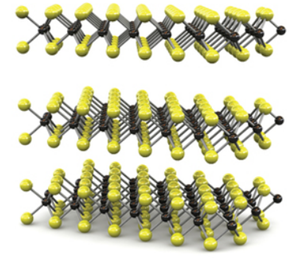
\includegraphics[height=.9\textwidth,left]{3d}
		\label{crystal1}
	\end{subfigure}
	\begin{subfigure}{0.30\textwidth}
		%\centering
		\caption{}
		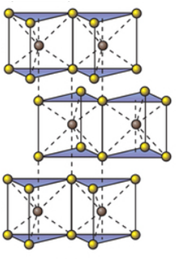
\includegraphics[height=.9\textwidth,center]{triangles}
		\label{crystal2}
	\end{subfigure}
	\begin{subfigure}{0.30\textwidth}
		\centering
		\caption{}
		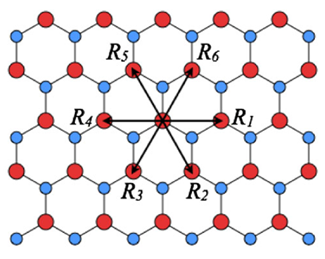
\includegraphics[height=.9\textwidth,right]{topview}
		\label{crystal3}
	\end{subfigure}
	\caption{Crystal structure of \tmds\!: \textbf{A} \tmds are composed of large sheets of transition metal atoms sandwiched in between chalcogenite atoms. Individual sheets are bound by strong in-plane covalent bonds and are being held together out-of-plane only by weak van-der-Waals forces. \textbf{B} In the 2\textsc{h} phase, the unit cell of \tmds has a triagonal prismatic shape with the transition metal in the center, between two triangles of chalcogenite atoms. \textbf{C} Viewed from the top, \tmds show a hexagonal lattice structure. However, because of the structure of the unit cell, the inversion symmetry is broken. Graphics from \cite{wang_electronics_2012, xiao_coupled_2012}}\label{crystal}
\end{figure}

Transition metal dichalcogenides (\tmds\!) belong to a class of materials that consist of large covalently bound sheets, that are held together by weak van-der-Waals forces. These so-called layered materials have gotten more attention since it has been shown, that individual monoatomic layers of them have unique properties, that are very different from the bulk material. The most prominent member of this group is graphene. Graphenes band structure shows what is called "dirac cones". This means that conduction and valence band touch at the $K$ point at the edge of the Brilloin zone, with the Fermi level seperating the two. The electronic dispersion relation in the vicinity of these "Dirac points" is linear. As a result charge carriers like electrons effectively behave like massless fermions, analogously to the linear dispersion of photons. This among other things causes very high electron mobility and conductivity. \textsc{Tmdc}s on the other hand are semiconductors and have long been known to have an indirect band gap. However, only since the discovery of graphene their properties in the limit of one atomic sheet---the monolayer---came into focus. 

Crystals of \tmds consist of a tri-atomic base of one transition metal atom like tungsten (W) or molybdenum (Mo) and two chalcogen atoms like sulfur (S), selenium (Se) or tellurium (Te). In nature these compounds can be found in lateral arrangement---a \tmdg monolayer (see figure \ref{crystal} \textbf{A}). \textsc{Tmd}s can exist in different metastable phases, that have a different crystal structure as well as different electronic properties \cite{ouyang_phase_2015}. The stable semiconducting phase is called 2\textsc{h}. In this configuration every transition-metal atom has six neighboring chalcogen atoms and forms a trigonal prismatic unit-cell, with the transition-metal in the center as depicted in figure \ref{crystal} \textbf{B}. A \tmdg monolayer exhibits a $\mathcal{D}^1_{3h}$-symmetry. The unit-cell is invariant under 3-fold rotation as well as in-plane reflection. In the top-view (see figure \ref{crystal} \textbf{C}) this looks similar to the hexagonal lattice structure of graphene, but with the key difference of a broken inversion symmetry. When the unit-cell is inverted with the transition metal atom as its inversion center, the chalcogen atoms wind up in empty locations as with any possible inversion point.

This has two important consequences, regarding the electronic band structure. As in graphene, the reciprocal lattice is hexagonal. At the $K$ points however, instead of the characteristic dirac cone, monolayer \tmds form a direct band gap in the visible range. Because of inversion symmetry breaking the degeneracy of the $K$ points is lifted. The two different $K$ and $K'$ points that are identical in graphene are distinguishable in \tmds and exhibit optical selection rules, coupling the valleys to light with opposite helicity. This circular dichroism gives rise to a new pseudo-spin degree of freedom---the "valley index". Analogous to electronics and spintronics, the term ``valleytronics'' has been coined to describe possible information processing by manipulating this property \cite{wang_electronics_2012, xiao_coupled_2012}. 

The valence and conduction bands of \tmds are formed by the hybridization of the $d$-orbitals of the transition metal with the $p$-orbitals of its six neighboring chalcogen atoms. More precisely, the first four conduction bands and the seven first valence bands are dominated by the five 5$d$ (4$d$) and 4$p$ (3$p$) orbitals of W (Mo) and Se (S) respecively, carrying 93\% of the total orbital weight \cite{cappelluti_tight-binding_2013,silva-guillen_electronic_2016}. At the $K$ and $K'$ points the valence band is formed mainly by the $d_{x^2-y^2}$ and $d_{xy}$ orbitals of the metal atom, that leads to large spin-orbit coupling that splits the valence bands by more than 150 meV  \cite{zhu_giant_2011}. This energy is large enough to suppress any transition between the two valence subbands even at room temperature. Because of time-reversal symmetry, the splitting is reversed in the $K'$ valley. With regards to optical transitions this results in tight locking of spin and valley degree of freedom. The conduction band---formed by the $d_{z^2}$ orbtial of the metal with some contribition from $p_x$ and $p_y$ of the chalcogen---exhibits much weaker but finite spin-orbit splitting, that leads to two distinct optical transitions $X$ and $D$, that will be explained later on.

\section{Excitons in \tmdg monolayers}\label{theory_exciton}

When electrons absorb photons of an energy higher than the band gap of a semiconductor, they gain enough energy to be elevated to the conduction band and are allowed to move freely throughout the crystal. Other electrons can hop to the vacancies making the holes just as free as excited electrons. They also effectively act like a positive charges, resulting in Coulomb forces between free electrons and holes. If this interaction is strong enough to overcome thermal excitation, the two quasiparticles can enter a bound state, called ``exciton''. In a bulk semiconductor electrons in between electron and hole weaken this interaction by screening the Coulomb interaction which results in a low exciton binding energy. The direct semiconductor \textsc{g}a\textsc{a}s for example exhibits an exciton binding energy of just 4.2 meV \cite{pelant_luminescence_2012}. Doing a rough calculation with $T=E_{binding}/k_B$ this corresponds to a temperature of 48 K, limiting exciton formation to temperatures well below that of liquid nitrogen.
The geometry of \tmdg monolayers however effectively reduces the screening effect. Because the movement of electrons and holes is confined to two dimensions, the electric field density in the material drops significantly and the strong Coulomb interaction between the free quasiparticles raises the exciton binding energy up to several hundred meV \cite{chernikov_exciton_2014, hanbicki_measurement_2015, he_tightly_2014}, corresponding to several thousand K in temperature. Therefore excitons can be excited at room temperature, which raises the possibility of exciton-based real-life applications. The Coulomb interaction results in an exciton Bohr radius of close to 1 nm and a very short lifetime in the order of picoseconds \cite{palummo_exciton_2015}. Hence, the recombination of excitons with emission of a photon is the most efficient optical decay channel and thus dominates the photoluminescence spectrum.
The decay also happens faster than the so called valley lifetime---the timescale of coupling between the valleys---preserving the helicity in their emission once they decay. This is called "valley polarization".
The thinness of \tmdg monolayers has additional implications. Since the electric dipole field of the exciton extends beyond the boundaries of the crystal, the dielectric environment has a big influence on the optical spectrum \cite{stier_probing_2016, borghardt_engineering_2017, jakubczyk_impact_2018}. Impurities such as microscopic water droplets or dangling bonds of silicon oxide can induce localized potentials, broadening the linewidth of the photoluminescence (\pl\!) features. This complicates spectroscopic studies. On the other hand, this high sensitivity could be used in quantum sensing applications to optically probe or visualize electric or magnetic proximity effects \cite{peng_valley_2017, zhao_enhanced_2017, smolenski_tuning_2016, neumann_opto-valleytronic_2017}.


\begin{figure}[t]
\centering
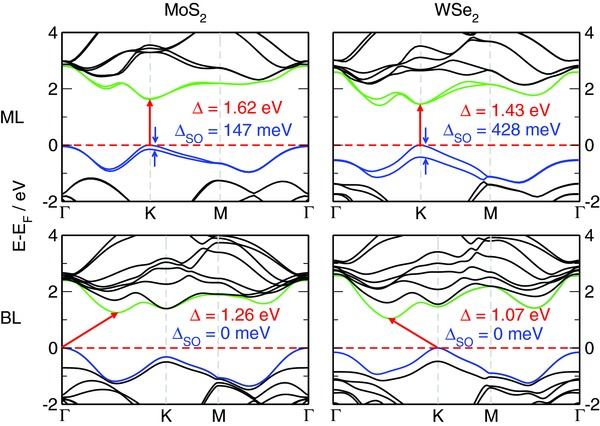
\includegraphics[width=.6\textwidth]{bandstructure}
\caption{Band structure for \mos and \wse mono- and bilayers calculated for room temperature. In the limit of a single atomic layer \tmds form a direct band gap at the $K$-point and the valence band is strongly split due to spin-orbit coupling. Graphic taken from  \cite{zibouche_transition-metal_2014_2}.}
\label{bandgap}

\end{figure}

\section{Optical spectrum of ws\textup{e}$_2$ monolayers}\label{composition}

\begin{figure}[t]
\centering
\begin{subfigure}{0.69\textwidth}
	\caption{}
	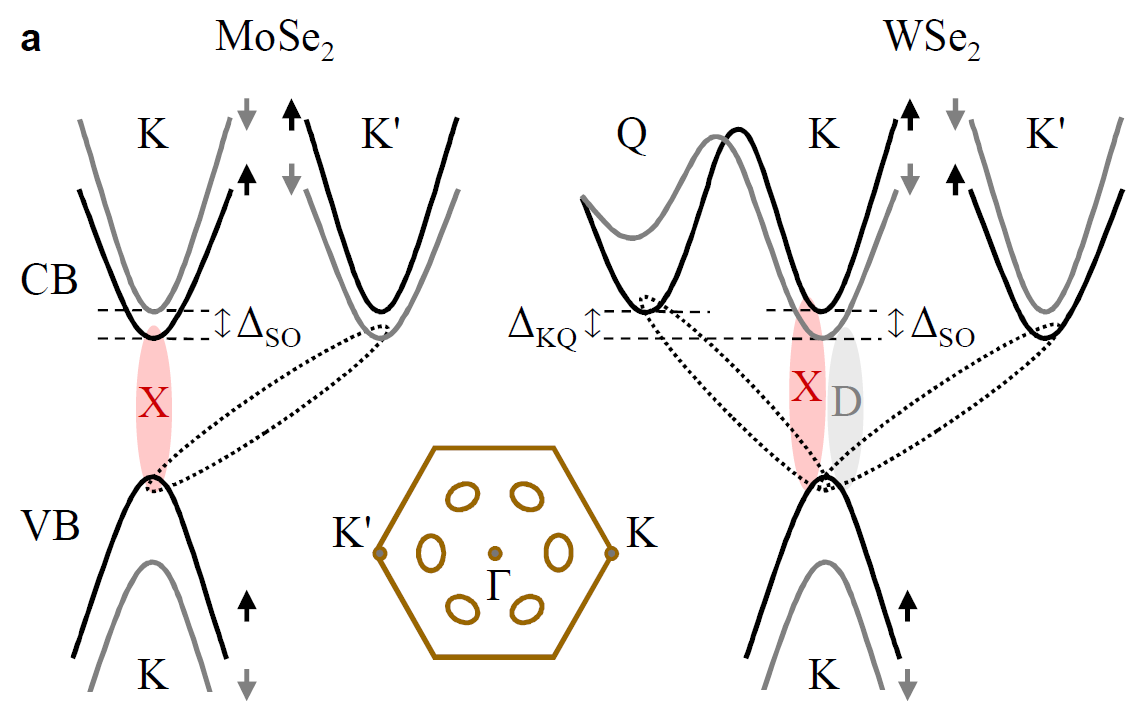
\includegraphics[width=.8\textwidth]{Band_structure_momentum_dark}
\end{subfigure}
\begin{subfigure}{0.3\textwidth}
	\caption{}
	\begin{tabular}{@{}rrrrr@{}}
	\toprule
	Mode&\Gamma&K&Q\\
	\midrule
	TA&0&15.6&11.6\\
	LA&0&18.0&14.3\\
	TO(E')&30.5&26.7&27.3\\
	LO(E')&30.8&31.5&32.5\\
	A$_1$&30.8&31.0&30.4\\
	\bottomrule
	\end{tabular}
\end{subfigure}
\caption{\textbf{A} Diagram of the band structure of \mose and \wse\! \cite{lindlau_identifying_2017}. In contrast to \mose the spin-like bright transition ($X$) in \wse does not have the lowest energy. Because of spin-orbit coupling, the $K$ valley with opposite spin is lower in energy, as well as the $Q$ and $K$ valley with parallel spin components. As a result the population of spin-forbidden and momentum-indirect excitons could be high enough to enable significant contributions to the \pl spectrum by these states, whose radiative decay is less efficient. \textbf{B} The 3-atomic basis of \tmds results in 3 accoustic and 6 optical phonon modes. Of these only 2 accoustic and 3 optical modes can couple to charge carriers. For $QK$ and $KK'$ indirect excitons phonons in the $Q$- and $K$-valley supply the right momentum to enable an optical transition and the formation of phonon sidebands. Their energies are theoretically calculated in  \cite{jin_intrinsic_2014} and given in meV. }\label{phonon_band}
\end{figure}

As stated above, the optical spectrum of \tmds both in reflection and \pl is dominated by the decay of excitons. In Tungsten-diselenide (\wse\!) the \pl spectrum shows a rich ensemble of characteristic spectral features, that so far have not been identified unambiguously. 

For \hbng encapsulated \wse the main exciton resonance ($X$) is located at around 1.72 eV, but the precise value can shift several meV, mainly because of strain \cite{zhu_strain_2013}. This resonance corresponds to the creation and annihilation of an exciton in the $K$ valley with electron and hole having a parallel spin component. The corresponding exciton with antiparallel spins is often called the dark state as its ``spin-forbidden'' ($D$). For symmetry reasons\textregistered\ its radiative decay is only allowed in-plane and spin-orbit coupling puts the state about 40 meV lower than the bright exciton \cite{echeverry_splitting_2016}. The \pl from these excitons can be collected from the side or with a high numeric aperture objective, that catches light not directly emitted out-of-plane \cite{robert_fine_2017, wang_-plane_2017}. In the presence of free charges---either holes or electrons--- excitons can interact with them to form trions that are associated with a redshift of 20-30 meV \cite{courtade_charged_2017}. While these properties can be predicted by modeling the trion as a three-body quasi particle, its precise nature still remains under discussion. The most contrarian interpretation to the helium-like bound state is a so-called fermi polaron. In a charged regime excitons behave like an impurity in a ``sea'' of electrons, forming the polaron quasi particle \cite{sidler_fermi_2016, efimkin_many-body_2017,schmidt_fermi_2012}.

The spectrum of \wse shows additional features, that have so far escaped thorough understanding. In light of strong sample-to-sample variation, they are commonly attributed to localized effects, like defect-induced quantum dots or local doping \cite{kato_optical_2014, zhang_defect_2017}, that create trapped excitons. Improved fabrication techniques like mechanical exfoliation and the usage of \hbng as a substrate (see section \ref{exfoliation}) have enabled experimentalists to measure spectra with very little defects and narrow linewidths, that still show a rich class of reproducible features.

\subsubsection{Phonon sidebands}\label{sidebands}

These peaks can be identified as phonon side-bands of momentum-indirect excitons \cite{lindlau_identifying_2017}. It has been shown, that in contrast to molybdenum-based \tmds \wse actually shows an indirect band gap \cite{zhang_probing_2015, hsu_evidence_2017}. As can be seen in figure \ref{phonon_band} \textbf{A}, the $Q$-valley lies energetically close to the $K$-valley and is believed to be located lower than the upper $K$-valley, that participates in the direct spin-like exciton transition. This could point to a high population of excitons composed of electrons in the $Q$-valley as well as in the lower lying spin-like $K'$-valley. While both these states are spin-allowed, momentum conservation prevents them from radiatively decaying in a single-photon process. Instead they can recombine with assistance of an additional phonon, carrying the inter-valley momentum. For momentum conservation to hold, the following equations have to be fulfilled for momentum-indirect excitons in the $Q$- or $K'$-valley respectively:
\begin{align}
	\vec{k}_K + (\vec{k}_K - \vec{k}_{Q/K'}) &= \vec{k}_K + \vec{k}_{photon} + \vec{k}_{phonon}\\
	\Rightarrow \vec{k}_{phonon} &\mbeq \vec{k}_K - \vec{k}_{Q/K'}
\end{align}
with $\vec{k}_X$ being a reciprocal lattice vector with momentum $X$. Because of the hexagonal structure of the Brilloin zone $\vec{k}_K - \vec{k}_{K'}$ simply equals a phonon in $K$ while $\vec{k}_K - \vec{k}_{Q}$ is conveniently close to a phonon in $Q$. Crystal vibrations in \tmds can have three acoustic and six optical modes, but only two acoustic and three optical modes can couple to charge carriers. This leaves a total of five possible phonon sidebands for both $Q$- and $K'$-indirect excitons, neglecting processes involving more than one phonon. Corresponding theoretically calculated energies can be found in \ref{phonon_band} \textbf{B} \cite{jin_intrinsic_2014}. 

Phonon sidebands appear as a peak redshifted by these energy values. For $K'$-indirect excitons the positions of the peaks can be inferred directly, since the energy splitting between the spin-like and spin-unlike exciton is known and both features can be measured. The $Q$-valley however has no direct decay channel. Therefore, its energy has to be deduced from its sidebands.


% \cite{van_der_donck_excitons_2018} 

\section{The valley zeeman effect}\label{zeeman}

%\begin{figure}[t]
%\centering
%\begin{subfigure}{0.99\textwidth}
%	\begin{tikzpicture}
%	\node[above right] (img) at (0,0) {\includegraphics[width=\textwidth]{valleyzeeman}};
%	\node at (60pt, 160pt) {$E_S$};
%	\node at (140pt, 105pt) {$E_S$};
%	\node at (26pt, 160pt) {$E_{\mathrm{orb}}$};
%	\node at (340pt, 70pt) {$E_S$};
%	\node at (390pt, 155pt) {$E_S$};
%	\node at (390pt, 70pt) {$E_{\mathrm{orb}}$};
%	\node at (253pt, 200pt) {$K$};
%	\node at (165pt, 200pt) {$Q$};
%
%	\end{tikzpicture}
%\end{subfigure}
%\caption{Diagram of orbital and spin contributions to the valley Zeeman effect. For excitons with parallel spin, the corresponding shift $E_S$ of conduction and valence band cancels out. The shift for the direct spin-like exciton therefore depends mostly on the magnetic shift of the orbitals $E_{\mathrm{orb}}$ that at the $K$ point is non-vanishing only in the valence band. The spin-unlike direct exciton however has a strong spin contributioin which in theory doubles its $g$-factor. For momentum-indirect excitons in $Q$ the $g$-factor almost entirely due to the difference in effective mass between hole and electron, because both $E_S$ and $E_{\mathrm{orb}}$ shift in the same direction in the conduction and valence band.}
%	\label{flakes}
%\end{figure}

%\begin{figure}
%	%\centering
%	\resizebox{!}{70pt}{%
%	\begin{tikzpicture}[scale=0.32, every node/.append style={transform shape}]
%	\begin{circuitikz}
%		\draw (0, 0) parabola (4, 4);
%		\draw (0, 0) parabola (-4, 4);
%		\draw (10, 0) parabola (6, 4);
%		\draw (10, 0) parabola (14, 4);
%		\draw[line width=1mm, dash pattern=on 8pt off 6pt] (10, -2) parabola (6, 1.5);
%		\draw[line width=1mm, dash pattern=on 8pt off 6pt] (10, -2) parabola (14, 1.5);
%	\end{circuitikz}
%
%	\end{tikzpicture}
%	}
%	\caption{}
%\end{figure}

A splitting of spectral lines in presence of a magnetic field has been studied for over a hundred years and is called the Zeeman effect is named after the scientist first measuring it in the spectral lines of sodium. The shift of different energy levels in an atom is a result of the magnetic moment of the state, caused by its orbital angular momentum and spin. Solid crystals are large ensembles of atoms that merge atomic orbitals to form the electronic band structure. Likewise, this band structure can shift in a magnetic field just as orbitals of single atoms. The 2\textsc{d}-nature of \tmdg monolayers and their broken degeneracy of the $K$ and $K'$ point gives rise to a new phenomenon called the ``valley Zeeman effect''. It describes a shift in the band gap energy that is different for both valleys, leading to a splitting of spectral lines with different circular polarization \cite{srivastava_valley_2015, aivazian_magnetic_2015}. In the vicinity of the $K$ point the band structure is dominated by large $d$-orbitals of the transition metal atoms. The hybridized $d_{x^2-y^2} \pm id_{xy}$ orbitals give the valence band an oribtal angular momentum along $z$ of $l_z=2\hbar$ that leads to a magnetic dipole moment of $\mu_{K,orb}=2\mu_B$. The conduction band is primarily formed by the $d_{z^2}$-orbital that has no out-of-plane angular momentum and therefore no magnetic moment along $z$. This leads to an asymmetric shift in the conduction and valence band and therefore to a shift of the band gap energy. The \tmd-geometry confines electron movement to the 2\textsc{d} plane, forcing the magnetic moment to either point upwards or downwards out of plane. This direction is exactly opposite at the $K$ and $K'$ points, shifting the valence band energy, and thus the band-gap in opposite directions. The total orbital magnetic moment at $K$ has a value of $\mu_{K,orb}=2\mu_B$. For the bright spin-like exciton transition this leads to a valley splitting of $\Delta_{K,K'}=4\mu_BB_z$. The prefactor in this equation is often called the $g$-factor and is given in units of the Bohr magneton $\mu_B=e\hbar/2m_e$. As it turns out, this first simple result is already in good agreement with experimental studies (see chapter \ref{spectroscopy}). However, the main reason for this are that other contributions are small or cancel each other out, which is not generally the case. The main additional contributions are the spin of electron and hole and their respective effective masses. %For excitons that only involve charge carriers at the $K$ or $K'$ point, 
This leads to the following formula:

\[\Delta_B=g\mu_BB_z = 2\mu_BB_z\left[(\tau_{e, \mathrm{orb}}-\tau_{h, \mathrm{orb}})+g_e(S_e-S_h) + \left(\tau_e \frac{m_0}{m_e}-\tau_h \frac{m_0}{m_h}\right)\right]\label{geq}\]

The first part of this equation belongs to the angular momentum of the orbitals forming the band structure. In the conduction band this value is $\tau_{e, \mathrm{orb}}=\pm2$ for $Q/Q'$ while it vanishes for $K/K'$. Only the $K/K'$ valleys are involved in the valence band and as discussed above, their contribution is $\tau_{h, \mathrm{orb}}=\pm2$. The second term in \eqref{geq} corresponds to the spin component of electron and hole. The spin of each particle has a value of $S=\pm\nicefrac{1}{2}$ witch is multiplied by the single-electron $g$-factor of $g_e=2$. The last term represents the correction from the quasiparticle effective masses with $\tau_{e/h}=\pm1$ representing the opposite direction of the magnetic moment in $K/K'$ or $Q/Q'$.

In the spin-like direct exciton $X$, the observed $g$-factor of $g_X=4$ mostly stems from the orbital angular momentum. Parallel spin components cancel each other and the difference in the effective mass term is only minor. For the spin-unlike exciton $D$---all else being equal---the spins of electron and hole point in opposite directions. Neglecting the mass term, this yields a $g$-factor of $g_D=8$. Predicting the $g$-factor for momentum-indirect excitons is more challenging though, because the difference in effective mass plays a more important role when electron and hole are coming from different valleys. Calculating the effective mass at a point in $k$-space can be done using a variety of theoretical approaches as done for example in  \cite{rybkovskiy_atomically_2017} for the $K$-valley. Not including this term would result in a vanishing $g$-factor for the momentum-indirect exciton in $Q$. The data in section \ref{zeemanspec} strongly contradicts this simple calculation.

\section{Bilayer ws\textup{e}$_2$}\label{bilayer_theory}

\begin{figure}[t]
\centering
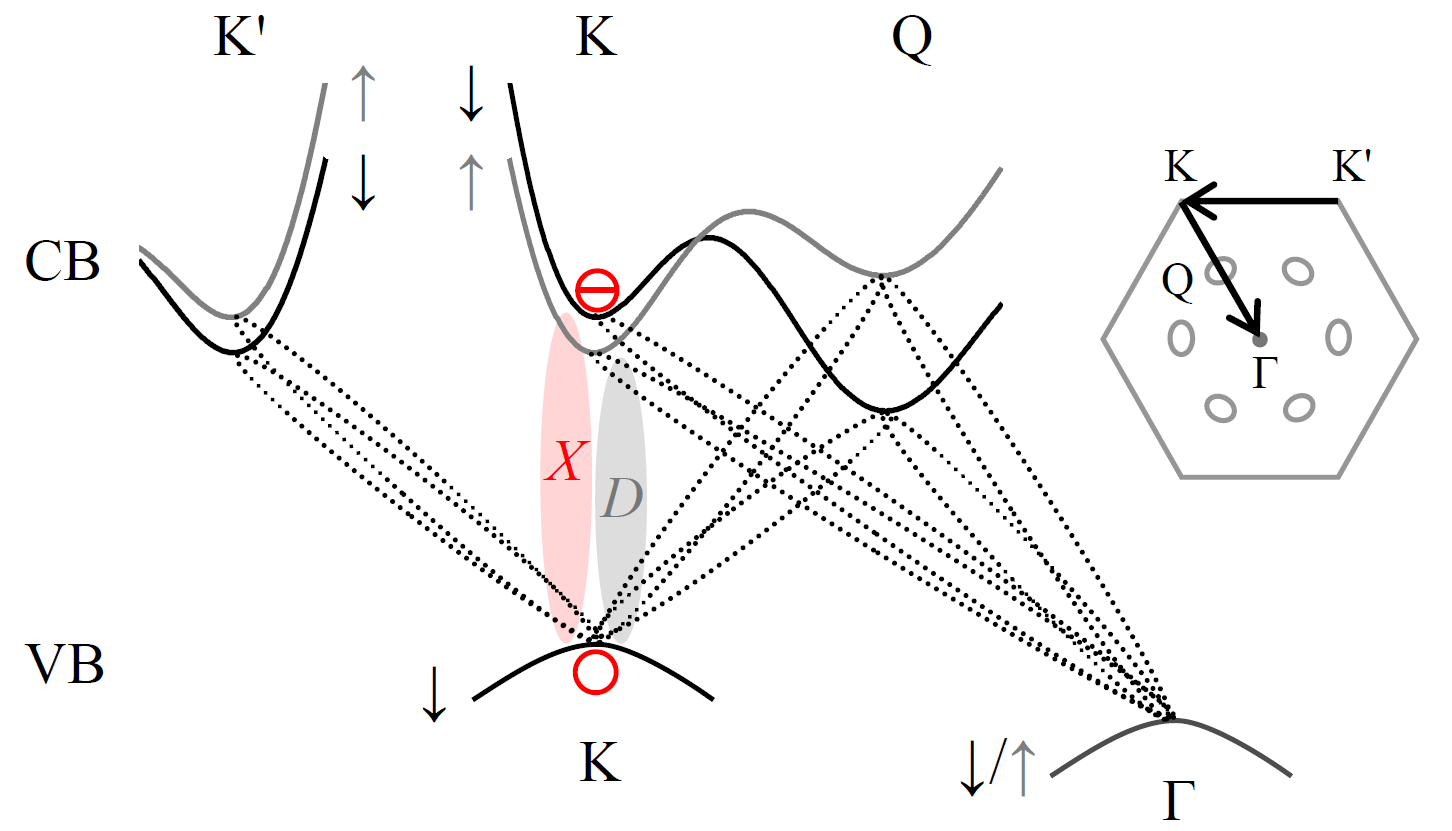
\includegraphics[width=.75\textwidth]{bilayerbands}
\caption{Bandstructure of bilayer \wse\!  \cite{lindlau_role_2017}. With respect to the monolayer the $Q$ valley in the conduction band drops significantly to form an indirect band gap with the $K$ valley. Additionally, the $\Gamma$ valley rises in the valence band, so that momentum-indirect excitions in $QK$ and $Q\Gamma$ become the energetically most favourable excitonic states.}
\label{bandgap}

\end{figure}

Even a single additional layer already fundamentally changes the properties of \wse\!. Inversion symmetry is no longer broken and the $Q$ valley drops below $K$ in energy, yielding an indirect band gap \cite{zibouche_transition-metal_2014_2}. Bilayer \wse is of particular interest because spin and valley degree of freedom are also coupled to the layer pseudospin, the location\red{noch ersetzen}s of the excited electron in one of the two layers of the sample \cite{jones_spin-layer_2014}. 

While in a bilayer the $K$ valley in the valence band is still at the highest energy, the $\Gamma$ valley is located only 40\pm30 meV below \cite{wilson_determination_2017}. Because the $Q$ valley lies lower than $K$ in the conduction band the majority of \pl of \wse bilayers originates from the decay of momentum-indirect excitons. \textsc{Pl} from the direct excitons involving electrons in $K$ ($X$ and $D$) yield much less intensity.

Momentum-indirect states can be composed of holes in $K$ and $\Gamma$ for the valence band and of electrons in $K$ and $Q$, with the $K$ valley's spin orbit coupling, splitting it in $K_\uparrow$ and $K_\downarrow$. In this notation $K_\uparrow$ is spin-parallel to the valence band in $K$ (see figure \ref{phonon_band} \textbf{A}). In the same way $Q$ is split into the lower lying $Q_\uparrow$ and the energetically higher $Q_\downarrow$. In the follwing, omitting the arrows will correspond to spin-up or spin parralel to $K$ in the valence band.

While combinations of all these valleys and their reversed counterparts could in principle contribute to the \pl spectrum, it is expected that the lowest energy states will have the strongest population and their phonon sidebands should yield the highest intensity in \pl\!. These are excitons coupling $Q$ in the conduction band and $K$ and $\Gamma$ in the valence band. The $QK$ and $Q\Gamma$ excitons are energetically close and it is not clear a-priori how they are ordered. According to measurements in  \cite{lindlau_role_2017} the latter one has the lower energy. 
%\chapter{Physical Properties of Transision Metal Dichalcogenide Monolayers}
\chapter{Fabrication of field effect structures}\label{exfoliation}

The main goal of this thesis was to implement a fabrication procedure for \tmdg monolayer samples, that yields narrow linewidth optical spectra and gate-tunability, enabling more accurate spectroscopic studies. This process builds on the work presented in \cite{funk_spectroscopy_2017}. Using the same mechanical exfoliation process in combination with standard contact lithography techniques and an advanced stamping procedure, this yields a fast and increasingly reliable process to build charge-tunable heterostructures of various \textsc{2d}-materials. 

\section{Mechanical exfoliation}
\begin{figure}
\centering
\begin{subfigure}{0.4\textwidth}
	\caption{}
	\begin{tikzpicture}
	\node[above right] (img) at (0,0) {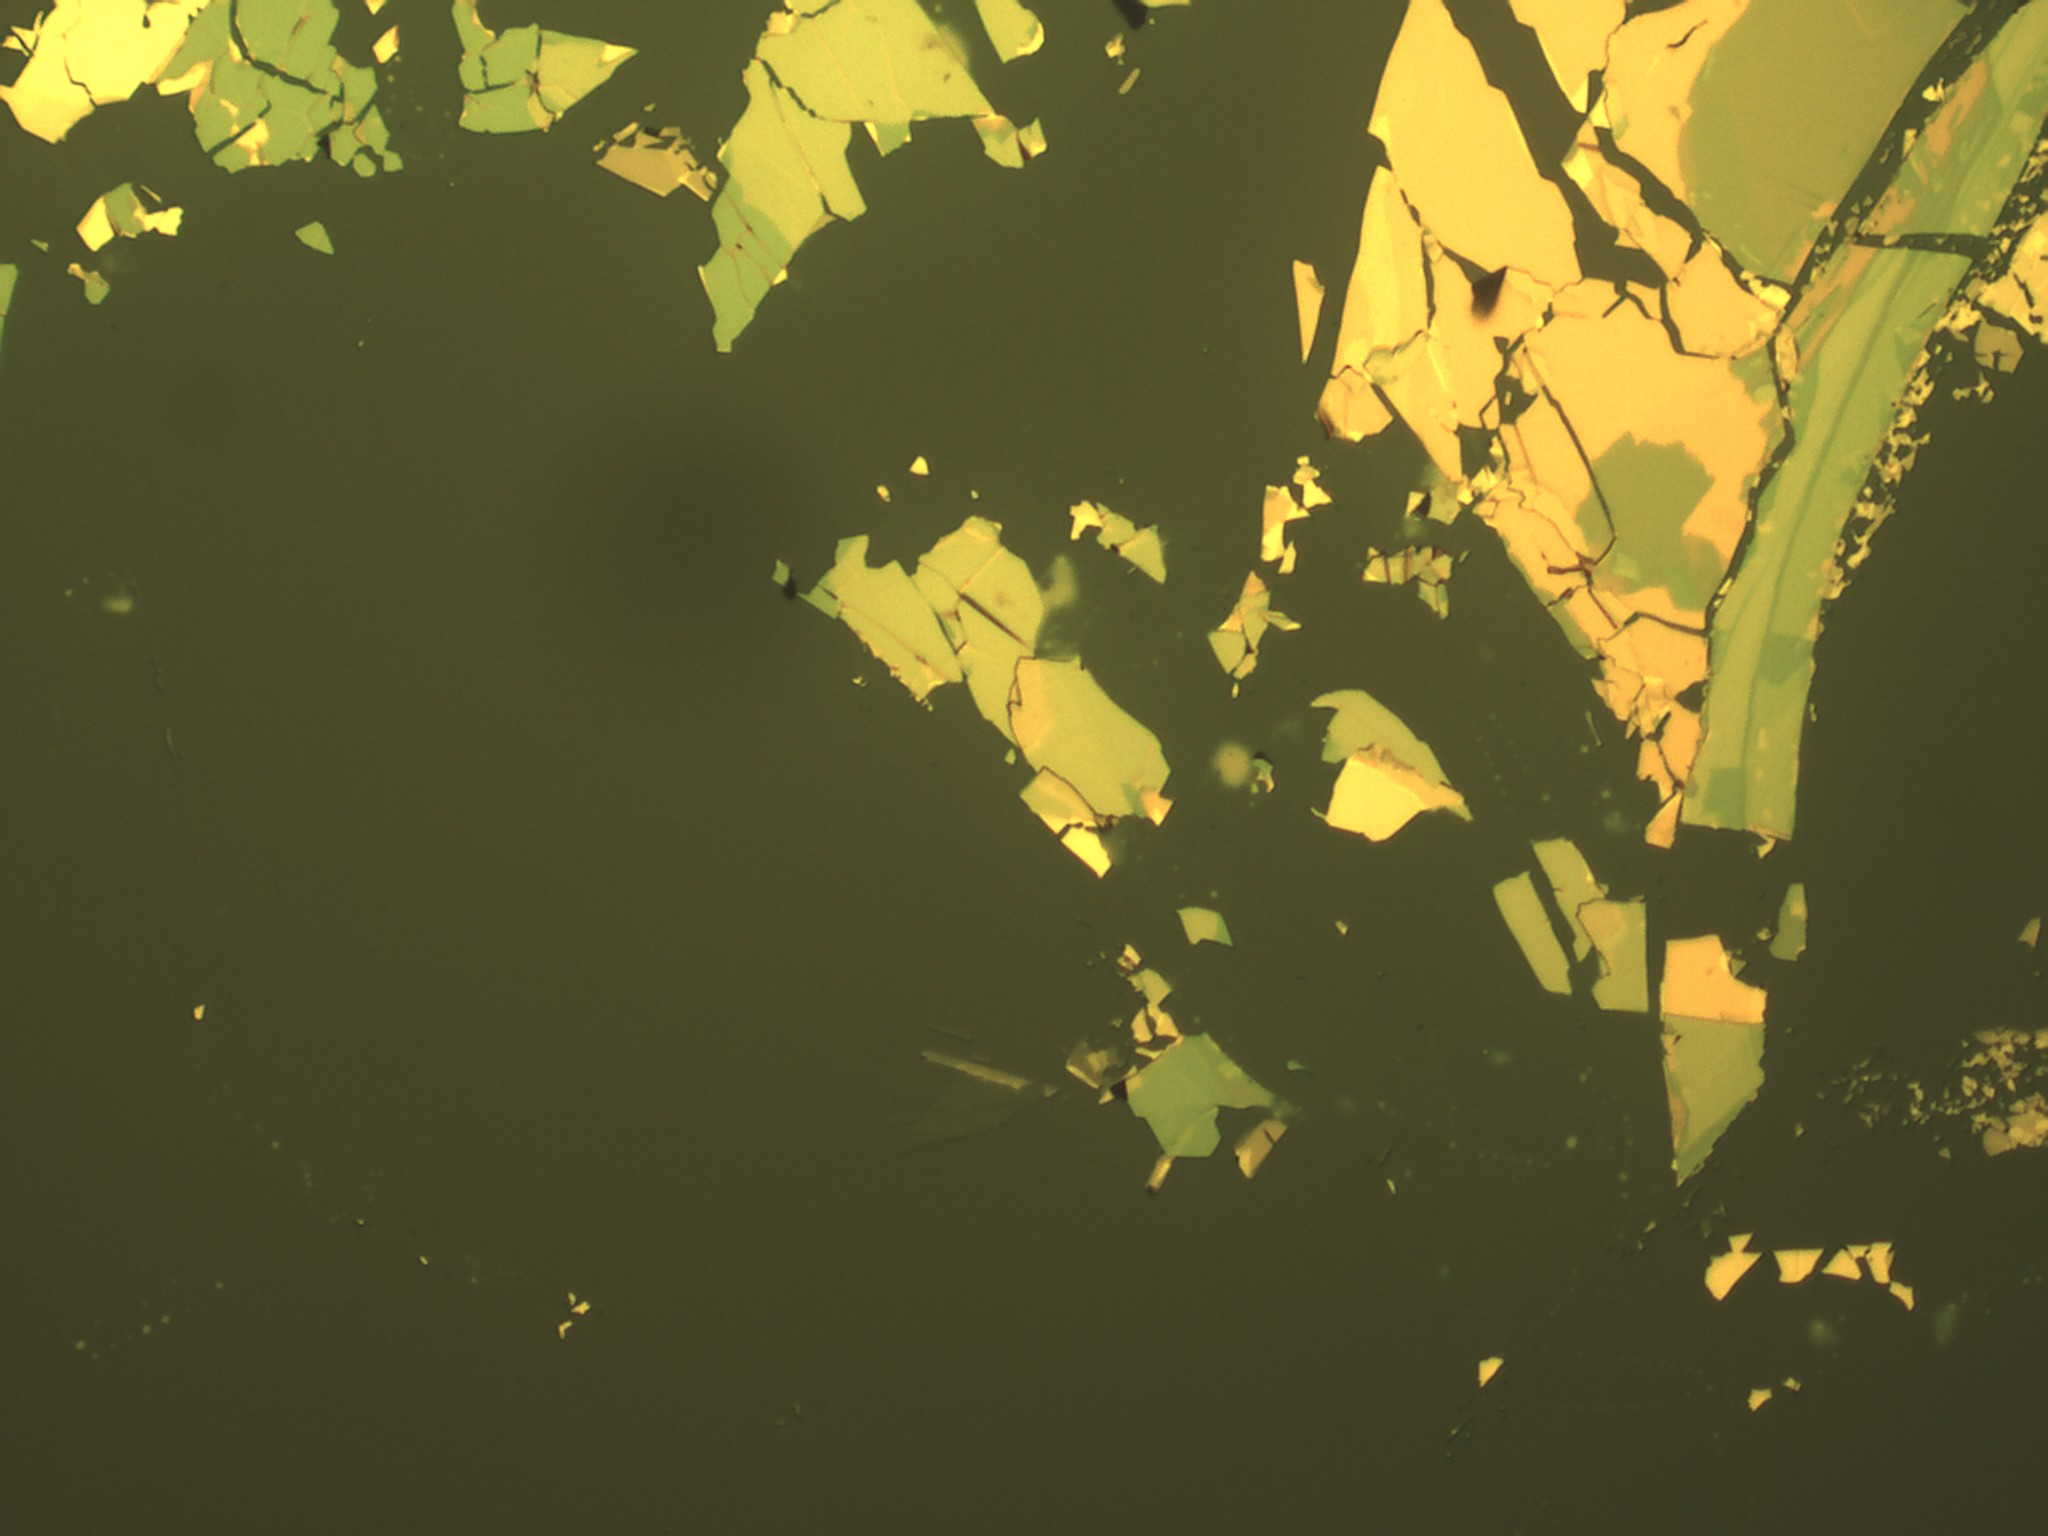
\includegraphics[width=\textwidth]{flakes.jpg}};
	\node at (84pt, 23pt) {{\large \textbf{ML/BL}}};
	\draw[red, dashed, thick] (83pt, 39pt) circle (9pt);
	\draw (20pt, 20pt) -- (60pt, 20pt);
	\node at (40pt, 12pt) {\textbf{100\mu m}};
	\end{tikzpicture}
\end{subfigure}
\begin{subfigure}{0.349\textwidth}
	\caption{}
	\begin{tikzpicture}
	\node[above right] (img) at (0,0) {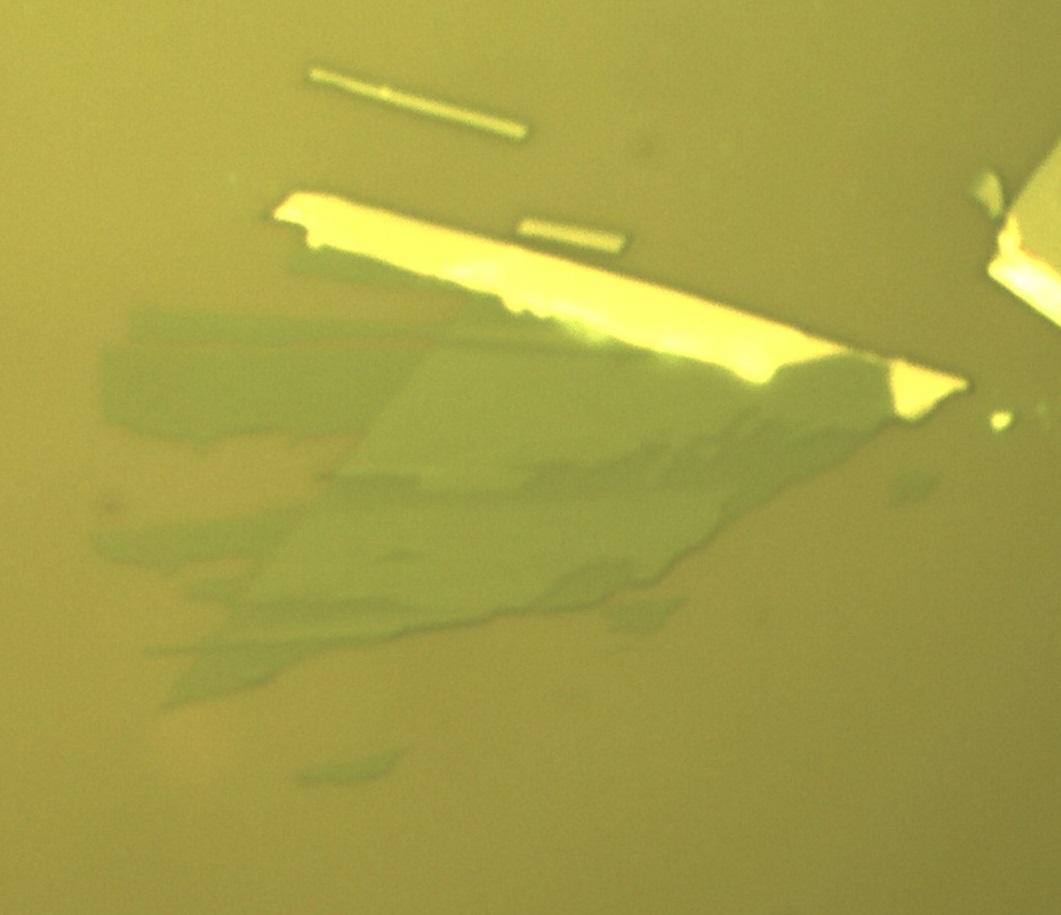
\includegraphics[width=\textwidth]{mono_on_sio2.jpg}};
	\node at (40pt, 80pt) {{\large \textbf{ML}}};
	\node at (65pt, 55pt) {{\large \textbf{BL}}};
	\draw (20pt, 20pt) -- (60pt, 20pt);
	\node at (39pt, 12pt) {\textbf{10\mu m}};
	\end{tikzpicture}
\end{subfigure}
\caption{\textbf{A} During the exfoliation process a lot of flakes of different size and thickness are scattered over the substrate. Interesting specimen have to be searched for by hand. \textbf{B} Flake consting of mono- and bilayer regions that can be identified by their optical contrast.}
	\label{flakes}
\end{figure}

Thin films of \tmds\!, like many natomaterials, can be fabricated using a top-down or bottom-up approach. The bottom-up method for \tmds is to grown single layers via chemical-vapor deposition (\textsc{cvd})\cite{chen_chemical_2016}. Because of its scalability it is the leading candidate for an industrial fabrication pipeline. However, the top-down approach of mechanical exfoliation has become the first choice for a lot of projects to build high quality model systems, that can be used to study physics in low dimensions\cite{geim_rise_2007}. The reason is the so far superior quality of few-layer flakes in terms of defects and contaminants as well as the synergy with dry transfer methods(See section \ref{hot_pickup}). 

The mechanical exfoliation process---often referred to as the ``scotch tape method''---leverages the fact, that the van-der-Waals forces between adjacent layers in \tmd's are much weaker, than the lateral covalent bonds---weak enough, that they can be easily broken apart by adhesive tape. The starting point is a solid crystal of \tmd-material, that can be produced either naturally or synthetically with high purity (supplied by hq-graphene). When a stripe of adhesive tape is brought in contact with it, a small amount can be peeled off. With a second stripe, that is put on the first one, the process is repeated multiple times. Each time the fresh tape is peeled of its parent, the strong adhesion between tape and \tmdg ensures a clean interface. Three to four repetitions are optimal to produce monolayers of a useful size. More repetitions further thin the material but heighten the risk of these thin films to break to smaller peaces, which complicates processing the flakes later on and build larger devices. 

To prepare monolayer flakes for the assembly of more complex devices, they first have to be transferred onto a suitable substrate. A standard substrate is silicon with a layer of thermal oxide that is between 50 and 90 nm thick. Before wafers of this material are brought in contact with the exfoliation tapes they are cleaned both in acetone and isopropanole before being exposed to oxygen plasma for 180 s. This ensures a clean surface and maximizes the material that sticks to the wafer(\cite{pizzocchero_hot_2016}). To release the tape the substrate is heated to 85°C for at least 2 minutes. After cooling down the tape can be peeled off and the wafer is inspected for monolayers. As seen in \ref{flakes}, this process yields a large number of flakes of different sizes and thicknesses on the substrate and it is common not to find a suitable monolayer sample on a typical \si-substrate (10 mm by 10 mm). 

\subsection{Layer number}

\begin{figure}
	\centering
	\begin{subfigure}{0.4\textwidth}
	\caption{}
	\begin{tikzpicture}
	\node[above right] (img) at (0,0) {\adjincludegraphics[trim={{.25\width} {.35\height} {.25\width} 0}, width=\textwidth, clip]{other_mono_bi.jpg}};
	\node at (80pt, 60pt) {{\large \textbf{ML}}};
	\node at (80pt, 150pt) {{\large \textbf{BL}}};
	\end{tikzpicture}
	\end{subfigure}
	\begin{subfigure}{0.4\textwidth}
	\caption{}
	\begin{tikzpicture}
	\node[above right] (img) at (0,0) {\adjincludegraphics[trim={ {.15\height} 0 {.1\height} 0}, width=.978\textwidth, clip, angle=90]{PL_imaging.png}};
	\node at (45pt, 45pt) {{\large \textbf{ML}}};
	\node at (100pt, 150pt) {\textcolor{white}{{\large \textbf{BL}}}};
	\end{tikzpicture}
	\end{subfigure}
	\caption{Comparison of mono- and bilayers of \wse\!. \textbf{A} The reflectance contrast of mono- and bilayers can be used to measure the layer number. The difference is however small enough to misidentify them under changing or inhomogeneous lighting conditions. \textbf{B} The \pl-intensity of the monolayer is almost an order of magnitude higher than the bilayer and can therefore be identified very easily.}
	\label{pl-contrast}
\end{figure}

Under an optical microscope (Olympus® - \textsc{bh}2-\textsc{uma}) monolayers can be identified using optical contrast and color as features to distinguish them from thicker films. It is possible to verify the layer number by these criteria alone using a camera and image analysis software\cite{funk_spectroscopy_2017}. However, this is much more reliable on transparent substrates, since the optical contrast is higher with an out-of-focus dark background. A reflective surface however enhances variations in the lighting conditions, making it harder to rely on absolute values of intensity. With our optical microscope and \si/\sio substrates, monolayer candidates where instead verified using photoluminescence (\textsc{pl}) imaging\cite{neumann_opto-valleytronic_2017}. In \tmds only monolayers show a direct band gap. Therefore even bilayers are much less efficient photonic emitters, showing almost an order of magnitude less \pl-intensity. The sample is excited with a laser with a wavelength above the direct exciton resonance and only the \textsc{pl} is collected on the chip of a \textsc{usb}-camera. A detailled description of the optical setup can be found in \ref{opticalsetup}. A sample measurement, comparing mono- and bilayer regions of \wse in a standard microscope image with \pl-imaging can be seen in figure \ref{pl-contrast}. 

Other methods to idetify monolayers inlcude both \pl and Raman spectroscopy\cite{zhao_lattice_2013,zhang_phonon_2015,tonndorf_photoluminescence_2013}. However, to fit in a fast assembly process \textsc{pl}-imaging proved to be the best method to verify the layer number as well the overall quality of the sample.

\section{Hexagonal boron nitride}

For spectroscopic studies of \tmds the right substrate plays a crucial part. As discussed in section \ref{theory_exciton}, the ultra-thin geometry of \tmdg monolayers makes them very sensitive to the dielectric environment. To obtain a narrow linewidth of the spectral features both in reflection and \pl spectroscopy, a suitable substrate has to fulfill some important specifications. A minimal surface roughness---ideally be atomically flat---avoids local modulation of the band structure through strain. Also, the substrate has to be dielectrically calm. These criteria rule out traditional substrates such as \si\ and \sio whose dangling bonds introduce localized charge defects, that introduce local variations in the potential landscape and inhomogeneously broaden spectral linres. In recent years hexagonal boron nitride (\hbn) has proven to be the superior choice to observe narrow linewidth spectra in \tmd's\cite{courtade_spectrally_2018}. \textsc{Hbn}, just like \tmds\!, is a layered material but belongs to the class of 2\textsc{d}-isolators, with a large, indirect band gap in the \textsc{uv}-range\cite{arnaud_huge_2006}. Thin, flat layers of \hbng can be mechanically exfoliated and achieve large, flat terraces. Few layers are sufficient to shield a \tmdg sample from the underlying substrate. To achieve even narrower lines, it can be ``sandwiched'' between two flakes of flat \hbng as was done with all samples contributing to this thesis. From the standpoint of fabrication \hbng has another important property. The van-der-Waals forces at \hbn-\tmdg interfaces are stronger than between \tmds and \sio\!. This is an important requirement for the hot pick-up assembly, discussed in section \ref{hot_pickup}.

\section{Electrode fabrication}

A gate-tunable \tmd-device can be understood as simple capacitor. A gate voltage is applied between the \tmd-flake and the doped \si\ substrate---separated by a 50 nm layer of thermal \sio\!. As in a normal capacitor, this voltage shifts the Fermi energy and results in free charges entering the two sides. In case of \tmds the voltage can also counteract intrinsic unintentional doping, by forcing free charges out the sample. Because \tmdg monolayers experience a varying degree of this intrinsic doping, this configuration is important to tune the sample to neutrality

\subsection{Top gate electrode}

\begin{figure}
\centering
\begin{subfigure}{0.4\textwidth}
	\caption{}
	\begin{tikzpicture}
	\node[above right] (img) at (0,0) {	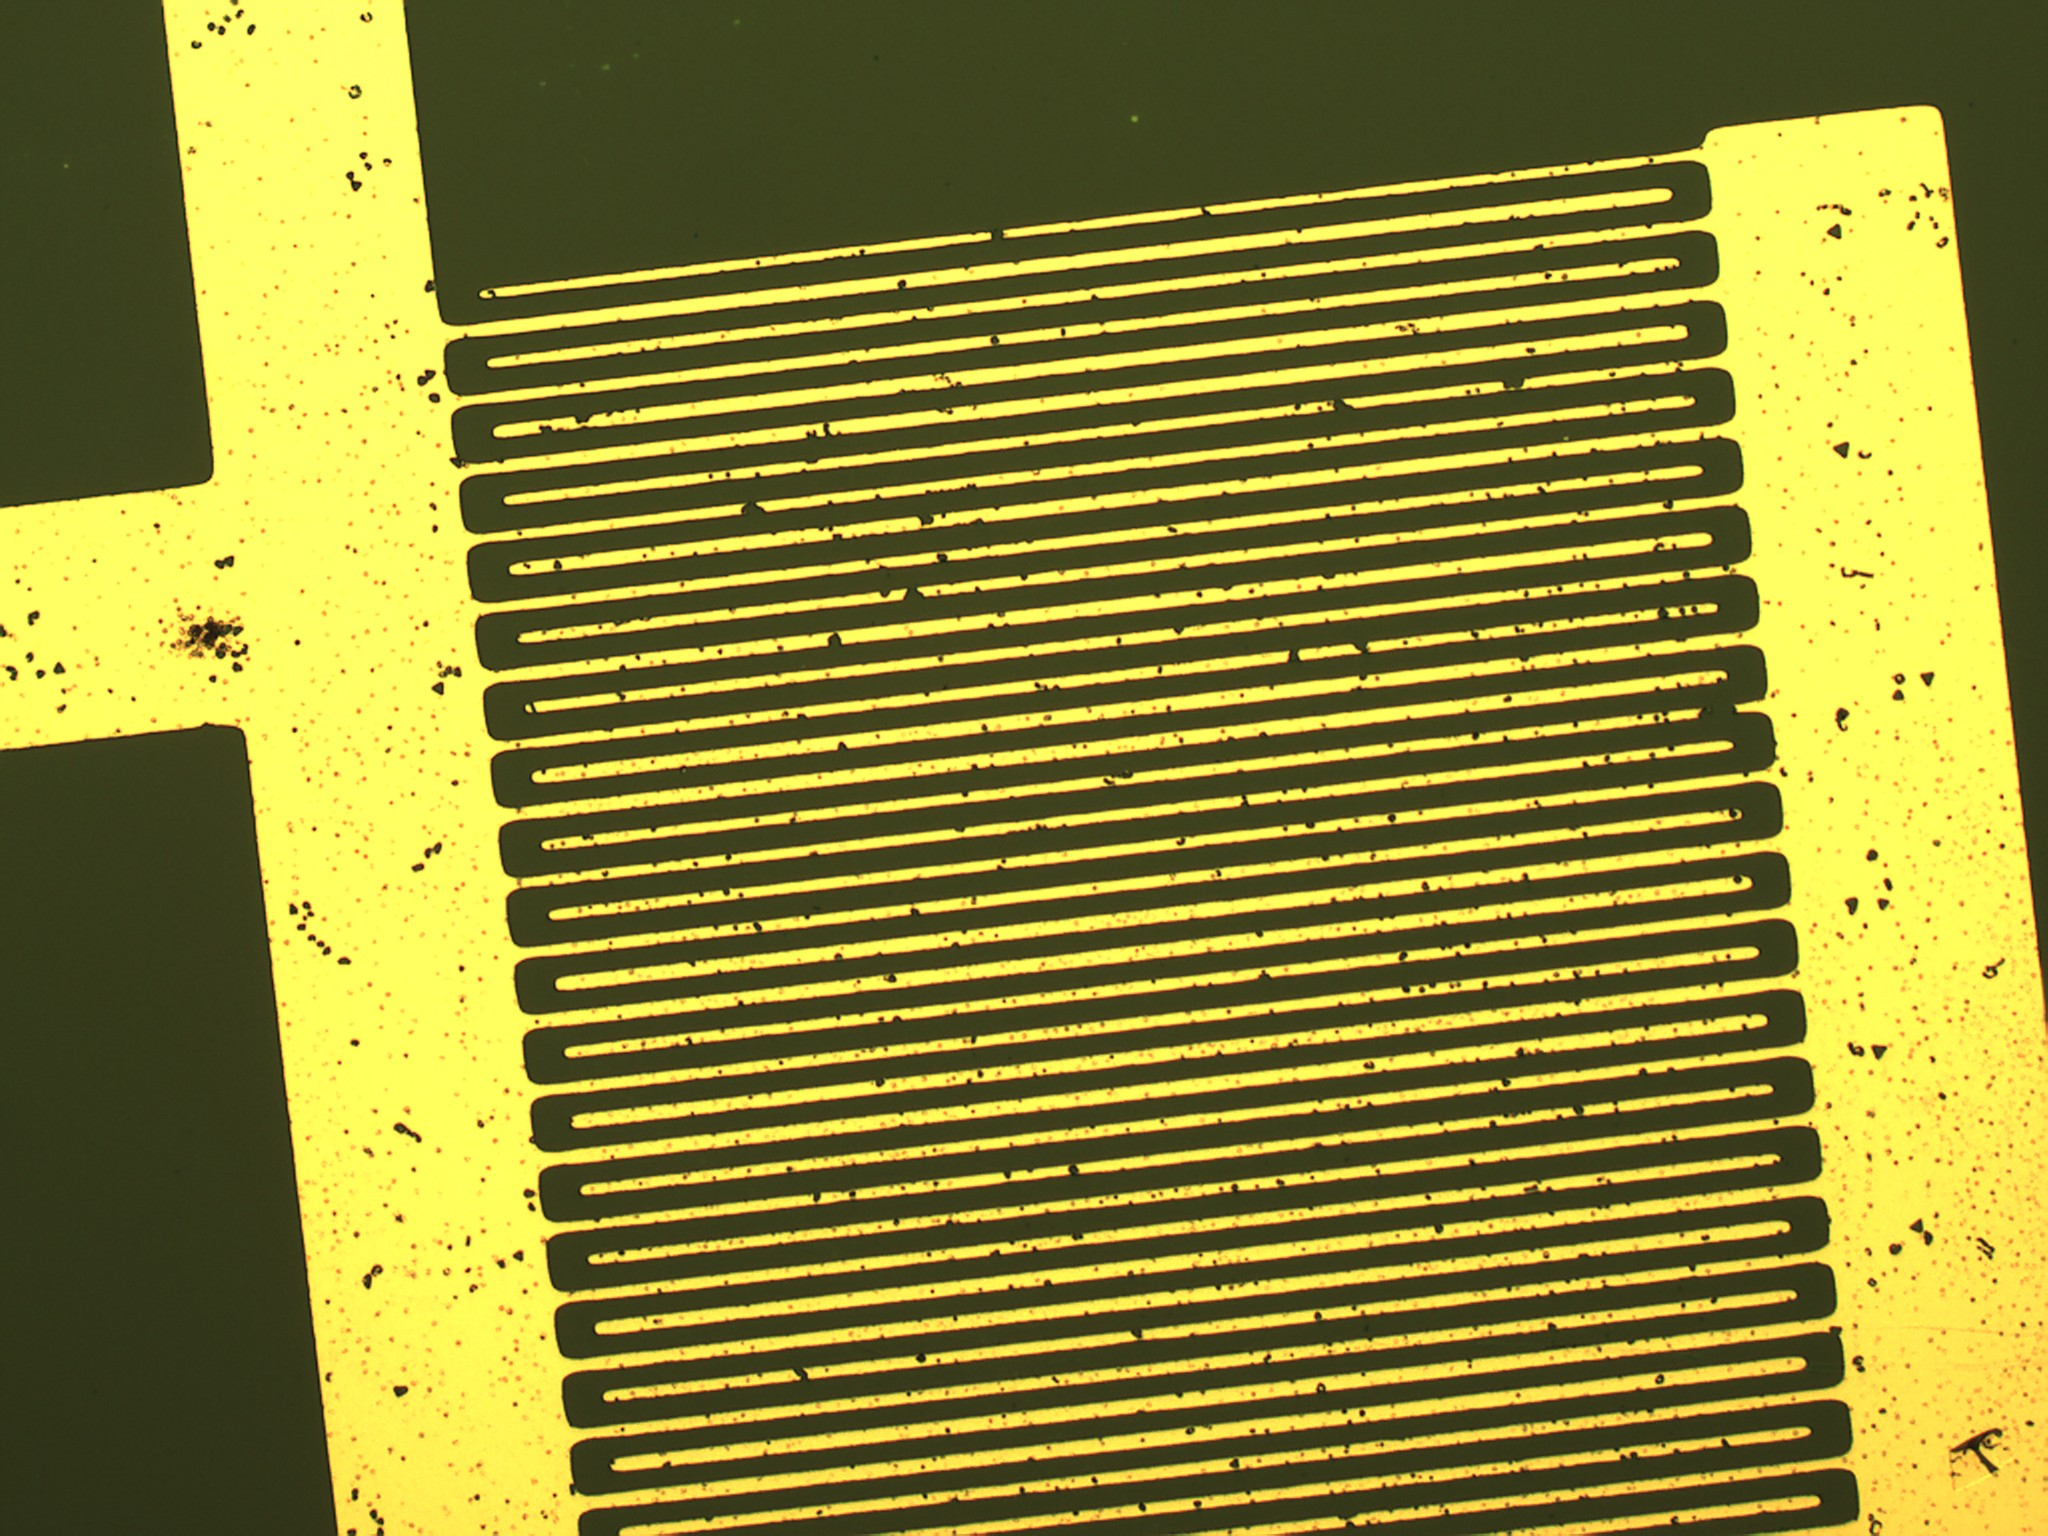
\includegraphics[width=\textwidth]{lithography.jpg}};
	\draw (20pt, 20pt) -- (60pt, 20pt);
	\node at (40pt, 12pt) {\textbf{200\mu m}};
	\end{tikzpicture}

\end{subfigure}
\begin{subfigure}{0.4\textwidth}
	\caption{}
	\begin{tikzpicture}
	\node[above right] (img) at (0,0) {	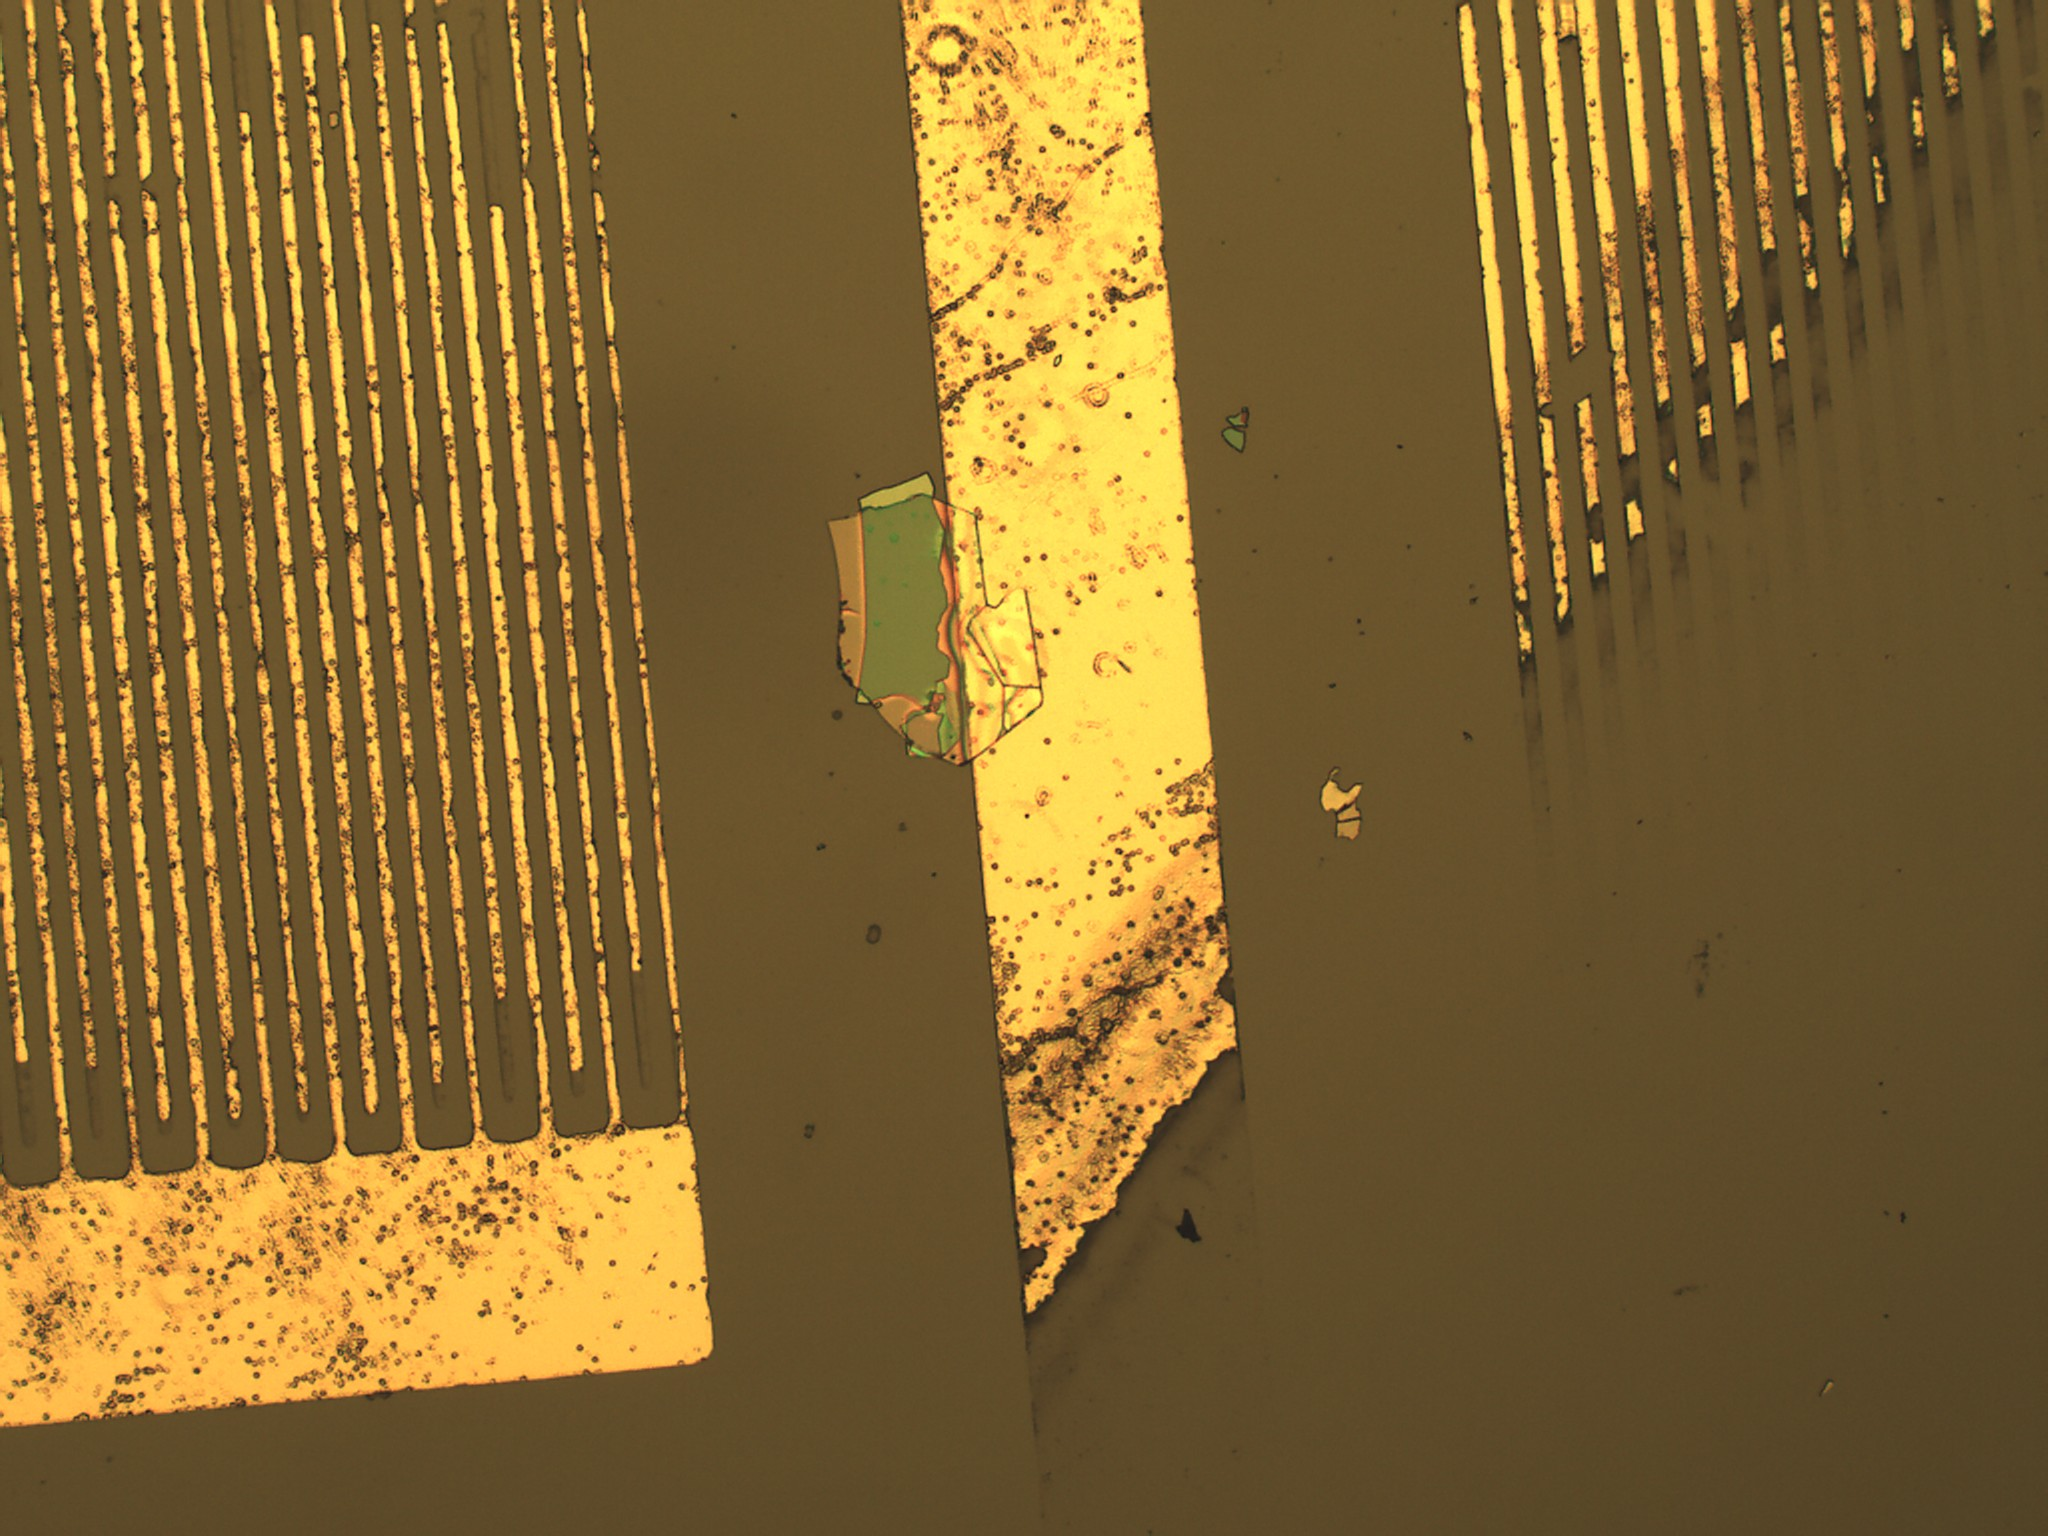
\includegraphics[width=\textwidth]{full_device.jpg}};
	\draw (120pt, 20pt) -- (160pt, 20pt);
	\node at (140pt, 12pt) {\textbf{200\mu m}};
	\end{tikzpicture}
\end{subfigure}
\caption{\textbf{A} Electrodes are written onto the substrate prior to the assembly of the \hbn-\tmdg heterostructure. A preused chromium mask of an interdigital structure is used for the gold pattern. \textbf{B} As long the heterostructure is dropped in contact with a thick line of the gold pattern, minor defects in the electrode structure do not affect the functionality of the device.}
	\label{pattern}
\end{figure}

To contact microscopic structures like \tmd-monolayers, electrodes have to be fabricated using micro-lithography. \textsc{Tmd} monolayers---either \textsc{cvd}-grown or exfoliated---are scattered on their substrates randomly. Therefore it is a common practice to fabricate electrodes directly on top of the sample via e-beam or laser lithography(Referenzen). Samples encapsulated in \hbng usually feature one or more additional films of graphene that provide an ohmic contact outside the heterostructure. Since only one contact is sufficient for charge-tunability, the process can be simplified greatly. Instead of writing electrodes after transfer, contacts are fabricated on the bare substrate. The encapsulated \hbn-\tmd-heterostructure can be contacted by dropping it on the edge of the gold structure. Most of the time, more \tmd-material than the monolayer is picked up during the transfer process. Because a \tmd-gold interface is conducting even at very low temperatures, these flakes provide suitable contacts, that do not have to be encapsulated in \hbn, therefore replacing additional graphene electrodes. Gold patterns are fabricated in contact lithography using a chromium mask that is deposited on glass. Because the stack can be dropped at any point on the substrate, the shape of the gold structure is unimportant, as long as it is large and connected. Therefore not even a new lithographic mask had to be fabricated. Instead a suitable mask was chosen from old pre-used structures. Even defects and deterioration of the masks only manifests aesthetically, rendering this process very robust and ideal for batch fabrication of gate-structures. The recipe starts with spin coating positive \textsc{az} 701 photoresist on a \si/\sio wafer. Using a maskaligner, the wafer is brought in contact with the chromium mask before exposing it to \textsc{uv}-light for 18 seconds. After that, the pattern is developed using \textsc{az} 826 \textsc{mif} developer, that washes out the exposed photoresist.

In the next step, the sample is coated in an X-ray evaporation system. First, a 1-5nm film of titanium is deposited on the substrate, that acts as a bonding agent. Subsequently a 50nm film of gold is deposited on top. After removing the sample from the vacuum chamber, the structures are finished in the so called ``lift-off''. The substrate is simply suspended in a solvent like acetone, that dissolves residual photoresist, only leaving gold, deposited in the developed. To speed up the lift-off process, the sample can be placed in an ultrasonic cleaner at a low power. The resulting structure can be seen in figure \ref{pattern}. 

\subsection{Back gate electrodes}

\begin{figure}
	\centering
	\resizebox{!}{150pt}{%
	\begin{tikzpicture}[scale=0.62, every node/.append style={transform shape},
        interface/.style={
        % The border decoration is a path replacing decorator. 
        % For the interface style we want to draw the original path.
        % The postaction option is therefore used to ensure that the
        % border decoration is drawn *after* the original path.
        postaction={draw,decorate,decoration={border,angle=-45,
                    amplitude=0.3cm,segment length=2mm}}},
        ]
	\begin{circuitikz}[american voltages]
		\draw (0,0) to[short] (0,0);
		\draw 
		(0,4) to[V, v=$20$V to $30$V] (0,0)
		(0,4) to[R, l=$3$k$\Omega$] (4,4)
		(0,0) to[short, *-] (4,0)
		(0,0) node[ground]{}
		(4,4) to[C, l=$1000$\mu F, *-*] (4,0)
		(4,4) to[short] (7,4)
		(7,4) to[short] (7,3)
		(7,3) to[short] (7.7,2.3)
		(7.7,2.3) node[inputarrow, rotate=315] {}
		(4,0) to[short] (7,0)
		(7,0) to[short] (7,1)
		(7,1) to[short] (7.7,1.7)
		(7.7,1.7) node[inputarrow, rotate=45] {}
		;
		\draw[line width=.5pt,interface] (8.1,0.7)--(8.1,3.2);
		\node at (8.2,3.6) {Substrate};
		\node at (6.8,2.05) {Gold wires};
	\end{circuitikz}
		
	\end{tikzpicture}
	}
	\caption{Circuit diagram for back gate fabrication: A capacitor is charged at 20V to 30V. Two boron-doped gold wires are moved very colesly to the silicon substrates. Once the distance between the wires and the substrate is low enough, an electric arc forms, discharging the capacitor through the substrate. Heat from the high current melts the tip of the gold wire locally doping the silicon and creating a gradient semiconductor/metal-interface.}\label{arc}
\end{figure}

Silcon is a semiconductor. A simple contact with a metal wire therefore results in a Schottky barrier at low temperatures. To create an ohmic contact to the backgate, the semiconcutor/metal interface is ``smeared out'' by diffusing boron doped gold into the substrate (see figure \ref{arc}). This is achieved by applying a high voltage between two gold wires and bringing them close to the substrate. Because the \si-substrate has a higher conductivity than the ambient air, an arc discharge between the tips of the wires will preferably find its way through the substrate. When the arc forms the tips of the gold wire evaporate and penetrate the \si-substrate. This creates a gradual metal-semiconductor interface and avoids a Schottky barrier, leaving a small gold droplet on the surface that can be contacted to a thin wire using conducting paste.

This process can be very violent. Gold droplets can splash over a large distance and evaporated gold can not only diffuse into the backgate but can also contaminate the \sio surface, lowering the breakdown voltage significantly. Therefore this step in the fabrication process should be taken before assembling the \tmd-\hbng heterostructure. This way, the substrate can be replaced in case of failure.

\section{Hot pick-up and transfer}\label{hot_pickup}

\begin{figure}
	\centering
	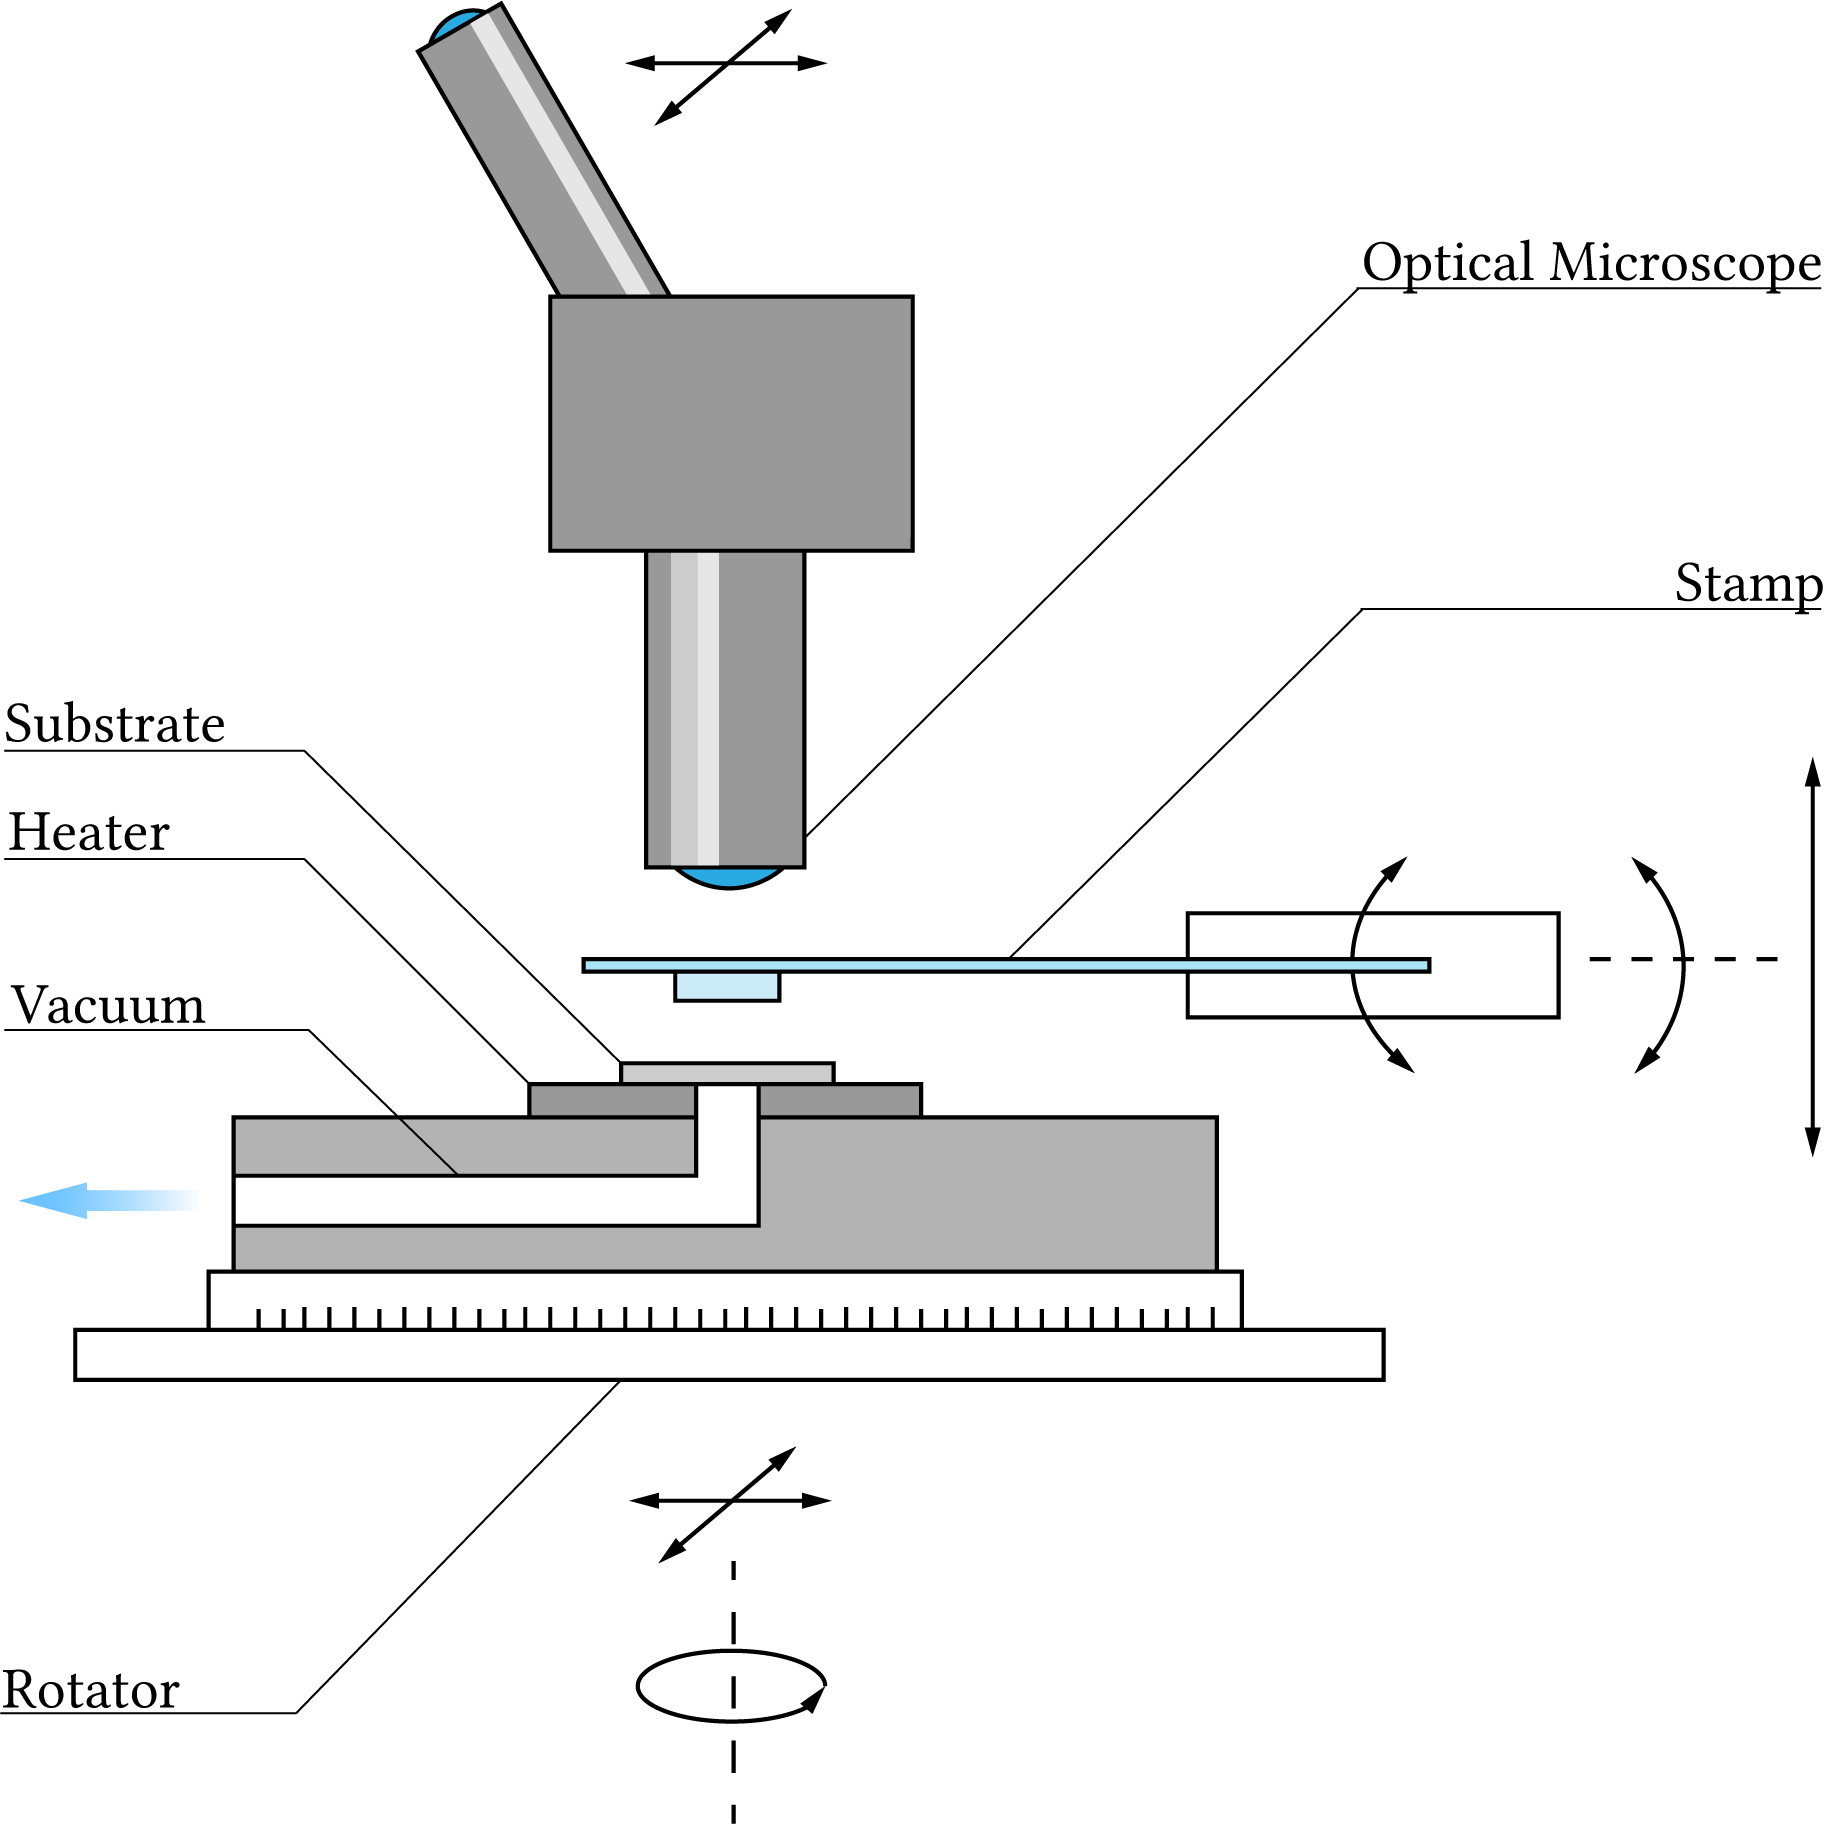
\includegraphics[width=0.7\textwidth]{Stempelaufbau.png}

	\caption{Setup for hot pick-up and stamping. The substrate is placed on a small, round \textbf{ceramic heater} with a 3mm whole in the center(Referenz Thorlabs), that is \textsc{pid}-controlled and can reach temperatures up to 200°C. It is mounted airtight onto the massive sample holder, that is connected to a \textbf{vacuum pump} to hold the \textbf{substrate} in place. It is \textbf{fully rotatable} and can be moved in plane. The \textsc{pdms/ppc} \textbf{stamp} is monted to a z-translator and can be tilted with respecto to both in-plane axes. The \textbf{optical microscope} can also be moved in-plane.}
	\label{stamping-setup}
\end{figure}


\begin{figure}[t]
\centering
\begin{subfigure}{0.49\textwidth}
 	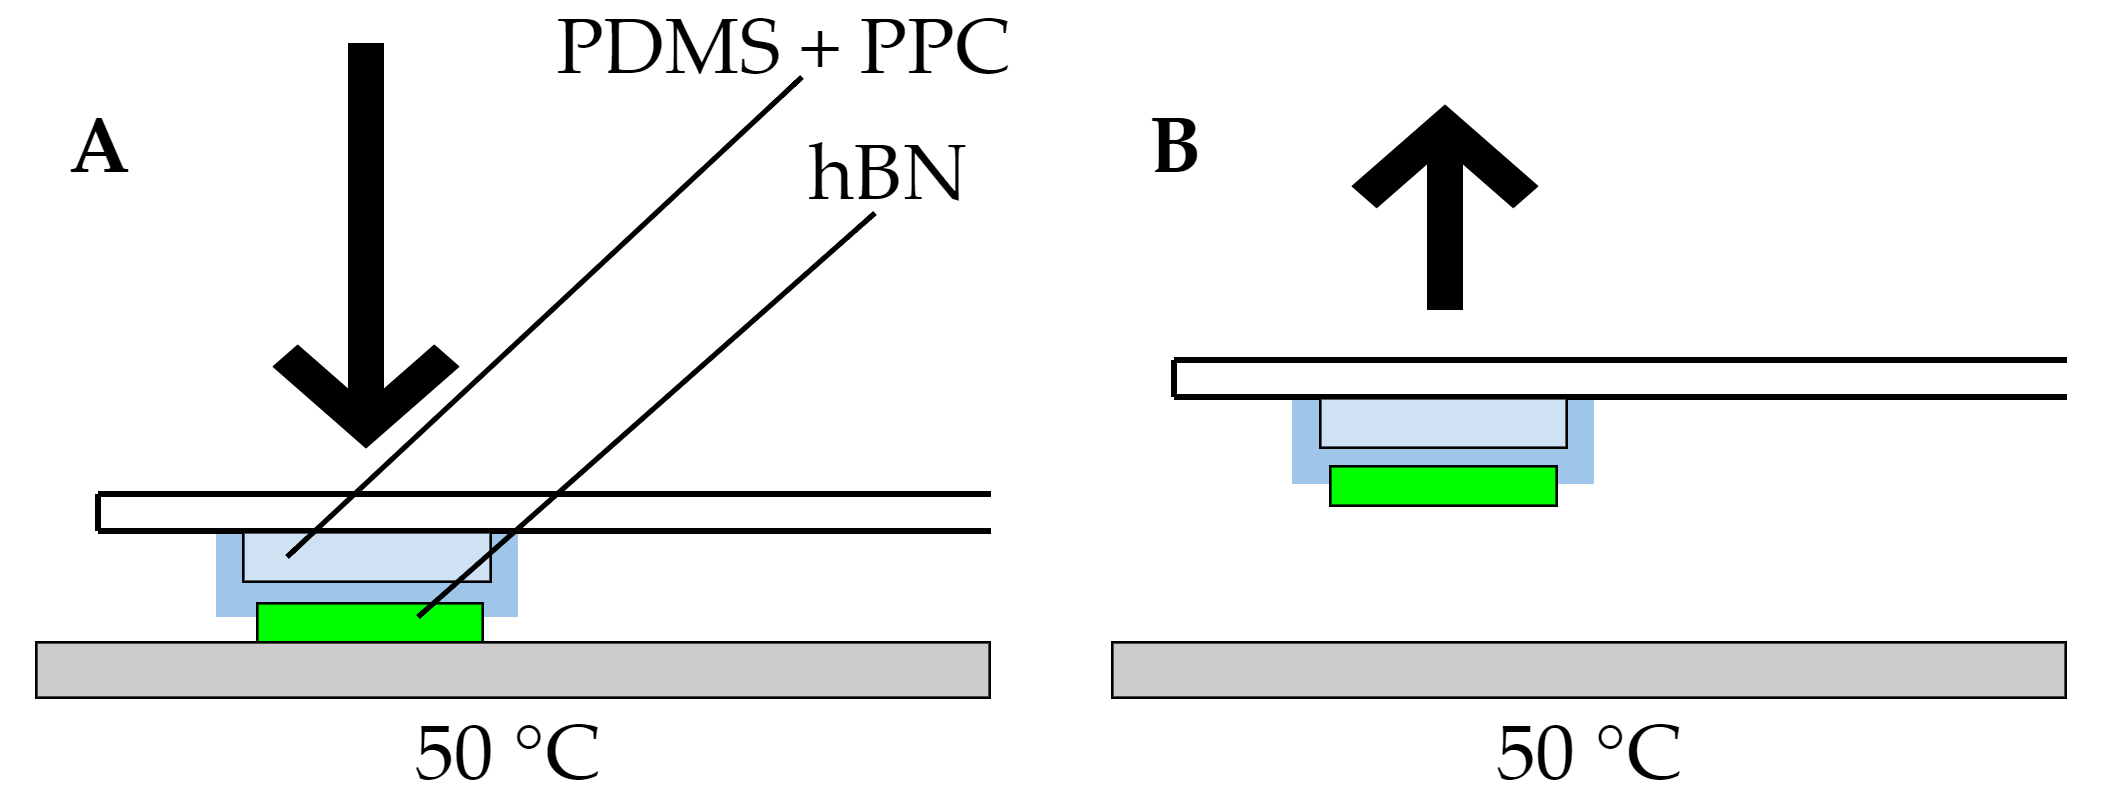
\includegraphics[width=\textwidth]{stamp_ab}

\end{subfigure}
\begin{subfigure}{0.49\textwidth}
	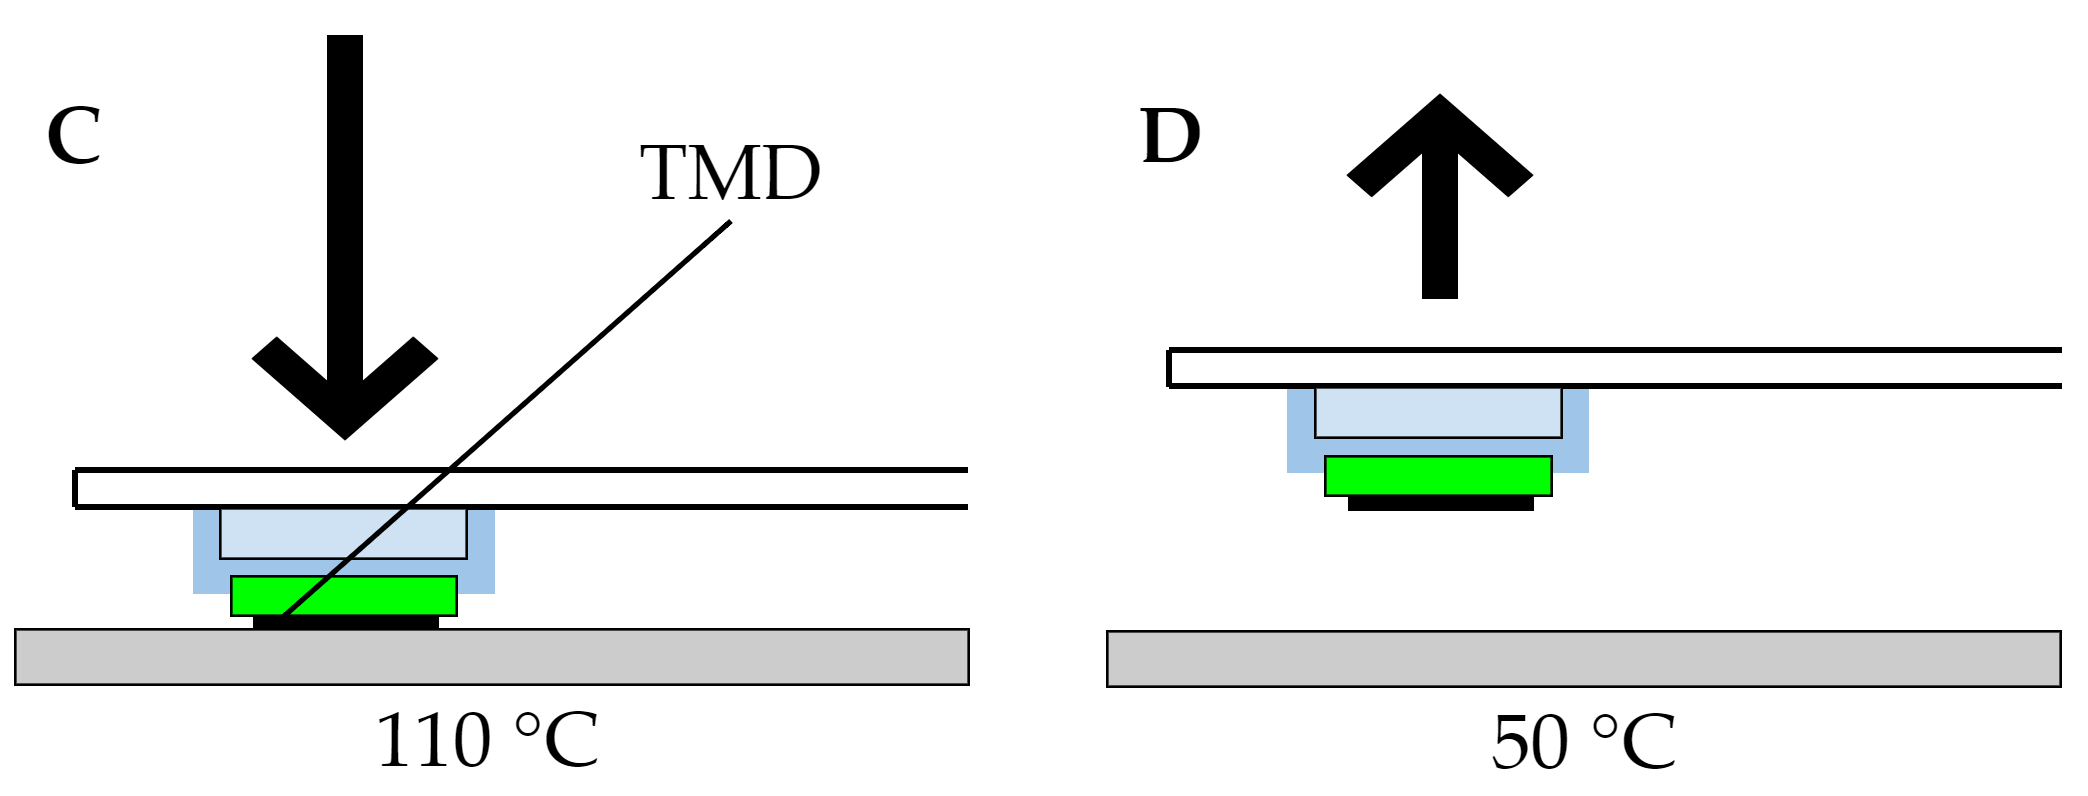
\includegraphics[width=\textwidth]{stamp_cd}
\end{subfigure}
\begin{subfigure}{0.49\textwidth}
 	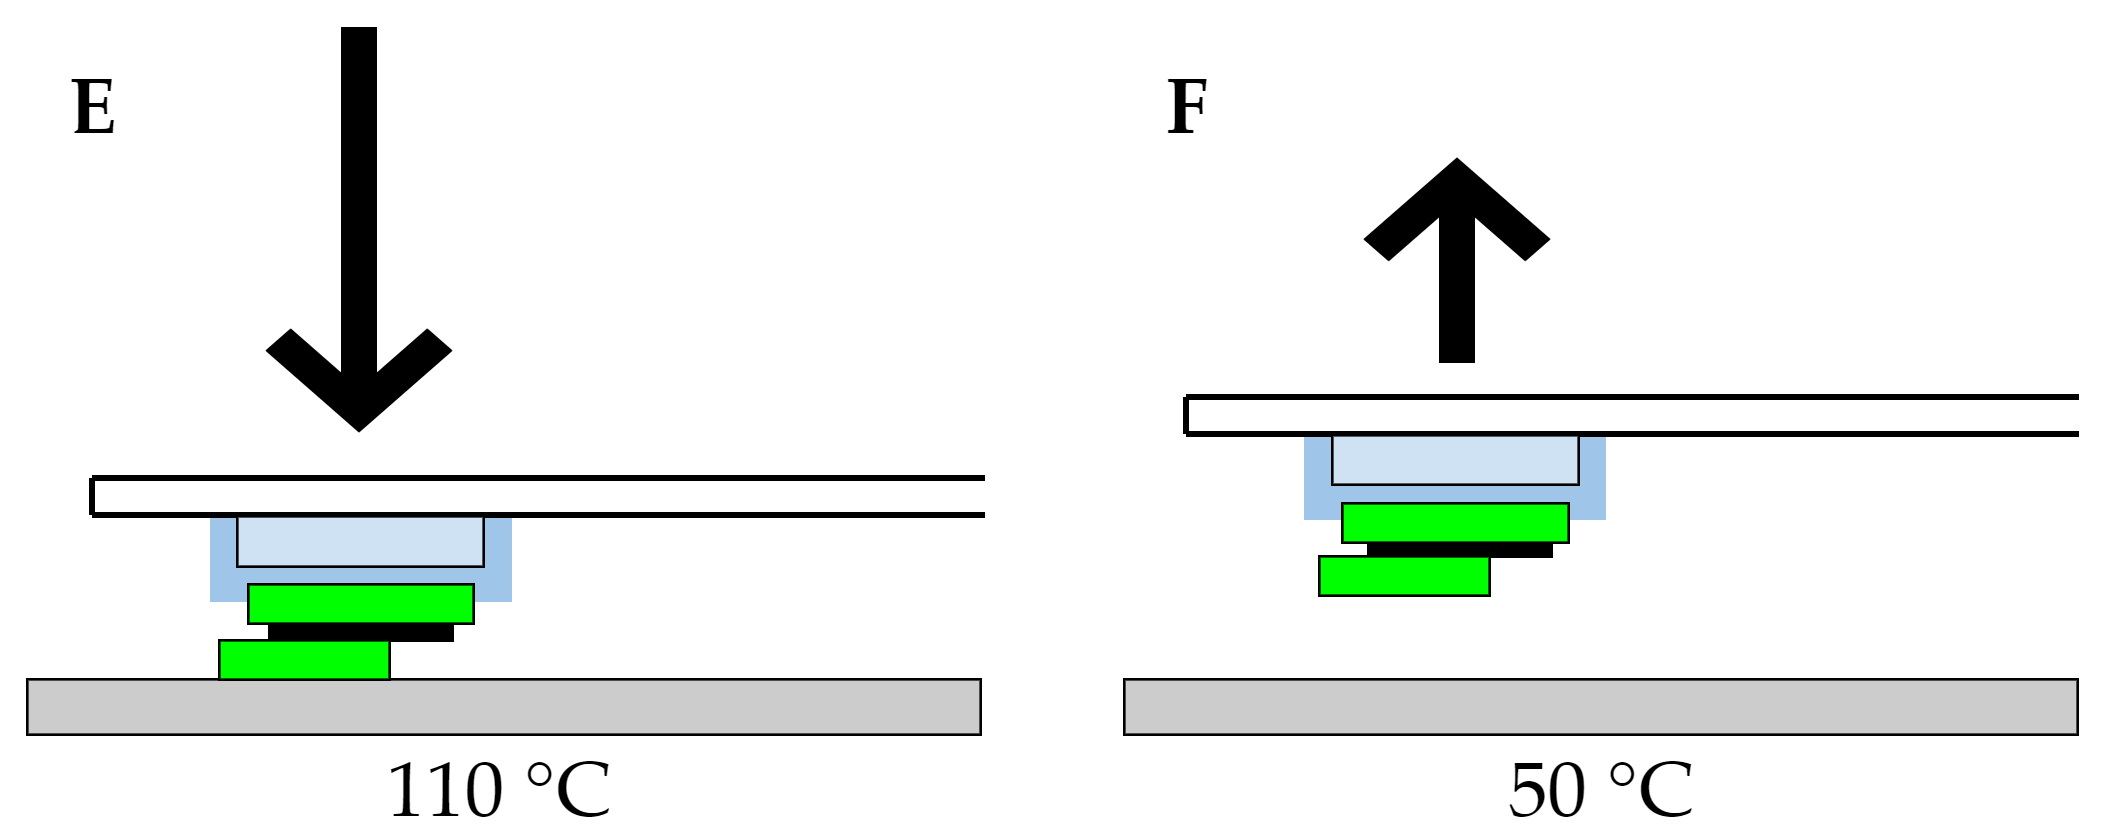
\includegraphics[width=\textwidth]{stamp_ef}

\end{subfigure}
\begin{subfigure}{0.49\textwidth}
	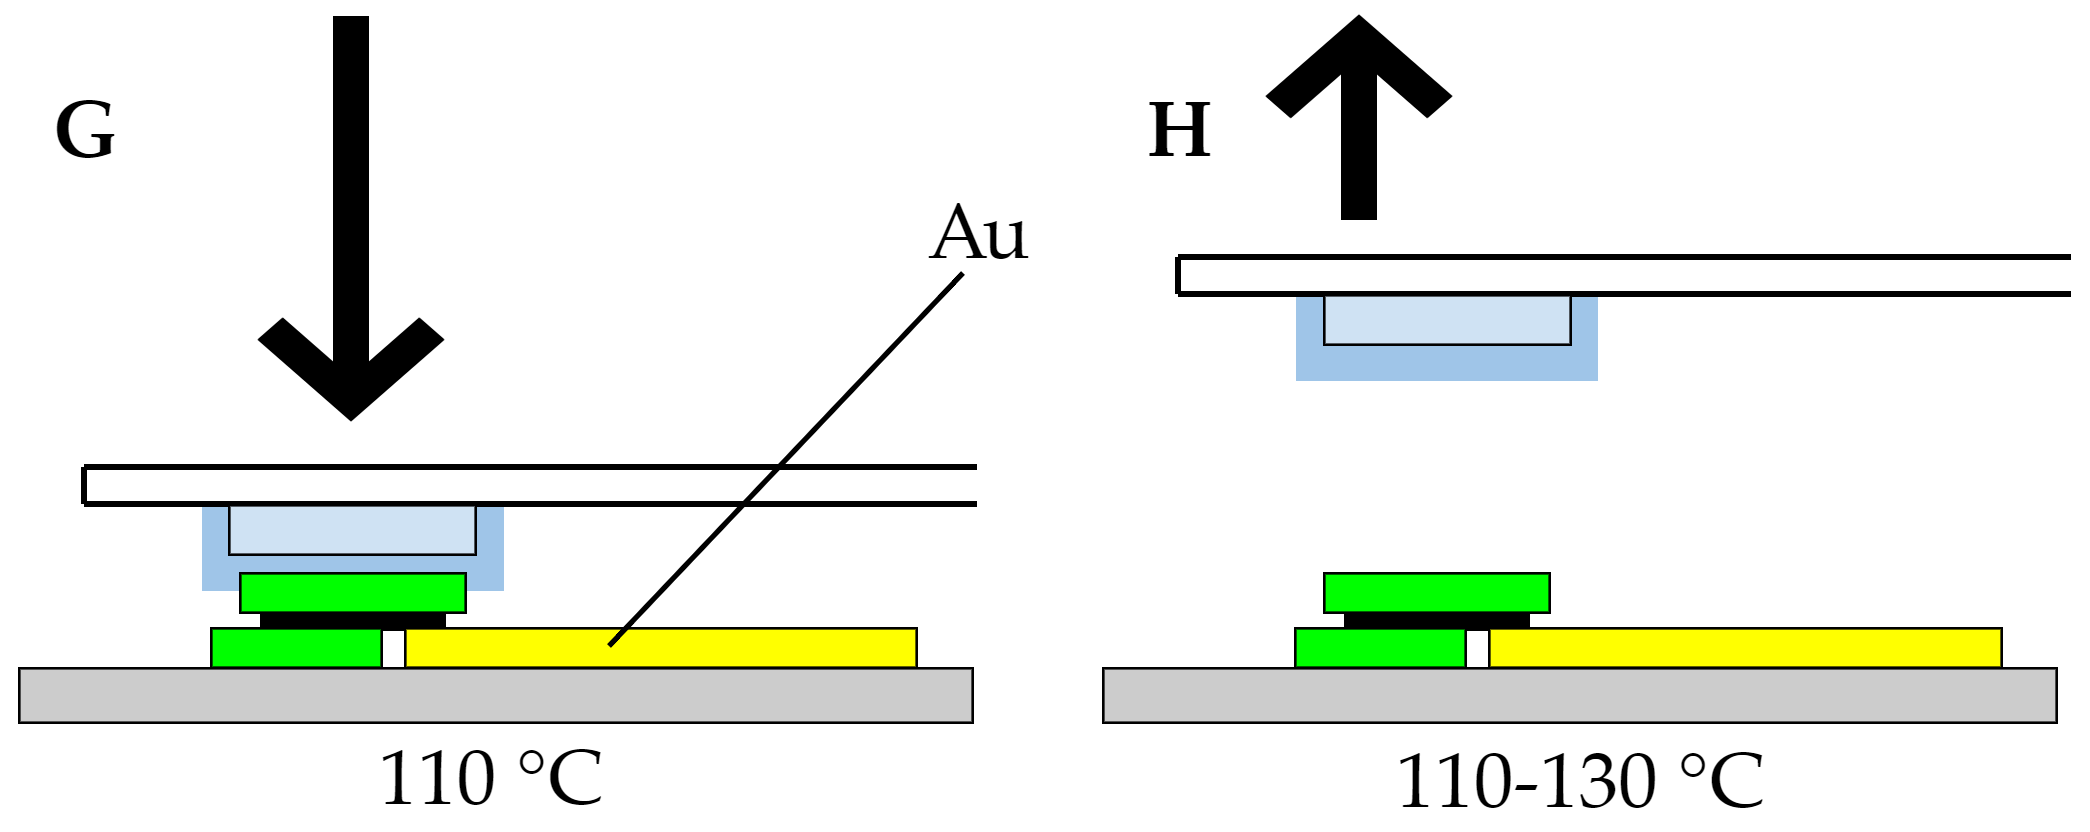
\includegraphics[width=\textwidth]{stamp_gh}
\end{subfigure}
\caption{Stamping process: "Hot pick-up and stamping" is based on strong van-der-Waals forces between \hbng and \tmds as well as the control of adhesion between \textsc{ppc} and \hbng using temperature. Flakes of \hbng are picked up from a \si/\sio substrate at 50 °C and can be dropped at a temperature around 110 °C, when the \textsc{ppc} film on the \textsc{pdms} block loses viscosity. Because thin \tmdg flakes like mono- and bilayers adhere to \hbng much better than to their substrate, the pick-up is highly reliable and arbitrarily high heterostructures can be built. To establish an electrical contact to a layer of the stack, part of it has to lay free, facing down. In this configuration the stack is simply dropped on the edge of the gold structure.}
	\label{stamping}
\end{figure}

The mechanical exfoliation method is popular also for its synergy with dry transfer methods. \textsc{Cvd}-grown \tmd-flakes are grown on suitible substrates and can be transferred to  a target substrate using a variation of wet methods, that involve powerful solvents or a combination of solvents and polymer films to lift the grown flakes off their initial substrate \cite{li_universal_2014}. The advantage of the exfoliation method in this regard is that flakes can be put on any substrate directly from the adhesive tape and do not encounter potentially damaging chemicals. This led to the invention of ``viscoelastic stamping'', where the \tmd-material is exfoliated on a substrate of viscoelastic polymer called polydimethylsiloxane (\textsc{pdms})\cite{castellanos-gomez_deterministic_2014}. This so called ``stamp'' can be brought in contact with the target substrate and peeled off carefully to drop down the flake at a desired position, opening up the possibility of producing carefully designed van-der-Waals heterostructures deterministically.

This method however can exclusively be used to drop \tmdg flakes, exfoliated directly on the stamp. This is limiting in a number of ways, since exfoliation on a polymer like \pdms\ comes with unavoidable contamination of the sensitive samples, that only gets worse with every new layer stacked on top. Attempts to develop more flexible methods to pick up \tmds and other 2\textsc{d} materials from clean substrates failed because van-der-Waals forces between the flake and a substrate like \sio could not be reliably overcome with a viscoelastic stamp. That is until \hbng was introduced as a more suitable substrate. It turns out, that van-der-Waals forces between \hbng and \tmds are high enough to remove them from \sio deterministically while a range of polymers can be used that strongly adhere to \hbng at an appropriate temperature.

This method is called ``hot pick-up and stamping''\cite{pizzocchero_hot_2016, tien_study_2016}. The stamp used in this process is a block of \textsc{pdms}, mounted on a glass slide with transparent adhesive tape. The active polymer however is polypropylene carbonate (\textsc{ppc}), that is spin-coated onto the \textsc{pdms}-block to form a thin, adhesive coating. \textsc{Ppc}, as a polar polymer sticks best to other hydrophilic substances. Therefore if the hydrophobic \textsc{pdms} is coated with \textsc{ppc} without additional treatment it can peel off, when in contact with \sio\!, especially at higher temperatures. However, the adhesion can be greatly enhanced by exposing \textsc{pdms} to oxygen plasma\cite{jung_adhesion_2016}. Before spin-coating all stamps were treated in a plasma-etching system (Gigaetch 3000) for 20 minutes, at 200 W of power.

The \tmdg and \hbn-flakes are exfoliated on a \si/\sio substrate. To raise adhesion with the flakes, these substrates are treated in oxygen plasma as well (180 s at 200 W). The primary criteria for finding the right \hbn-flakes is the flattness of its surface, so that the \tmd-flake can be encapsulated between two large terasses without cracks or steps. To allow a fast fabrication process, this flattness is only judged with help of an optical microscope. More sophisticated methods like atomic force microscopy can be used to verify the flatness more accurately. This is however much more beneficial, if the thickness of the \hbng plays an important role, for example when it is used in an optical microcavity \cite{sidler_fermi_2016}.

The goal of the hot pick-up is now to use a hot-plate to control the van-der-Waals forces between \hbn, \tmds and the substrate to ensure adhesion between the parts of the heterostructure as well as to reduce contamination with water molecules from the ambient air.

After all precursors are prepared on \si/\sio substrates, the actual pick-up and stamping process can be carried out. The fabrication setup can be seen in figure \ref{stamping-setup} and a the process in \ref{stamping}. The first step is the pick-up of the top \hbng flake. At 50°C the van-der-Waals forces between \hbng and \textsc{ppc} are already strong enough to lift the flake off the silicon substrate. Bringing flake and \textsc{ppc} in contact at a higher temperature can help as well, because this reduces the polymers viscosity. When cooling down to 40°C to 50°C afterwards, it becomes more rigid again and sticks to the \hbng more easily. In the next step the \hbng is dropped dropped on the \tmd-flake. At a higher temperature of 110°C \textsc{ppc} becomes almost fluid and peels off \hbng with ease. While the adhesion between thin \tmdg flakes and \hbng are strong enough to facilitate a pick-up also way below that temperature, heating the substrate during the drop helps to reduce the contamination with droplets of water. Since both \tmdg and \hbng flakes are prepared on clean wafers, humidity in the ambient air of the clean-room seems to be the biggest concern. Raising the temperature above the boiling point both minimizes the formation of actual droplets and also makes blisters of humid air and other contaminants at the \hbn-\tmdg interface more mobile. Dropping the stamp very slowly therefore helps to push these blisters out to the edge of the substrate\cite{pizzocchero_hot_2016}. The stack of \tmdg and \hbng can then be picked up again following the same procedure that was used for the bare \hbng flake. By repeating both steps of pick-up and drop-down an arbitrary number of layers can be added to the heterostructure. In this case it is dropped down on the bottom \hbng flake. To contact the \tmdg flake to gold part of it has to remain outside the \hbng encapsulation. This part does not necessarily have to be a monolayer but can also be any form of \tmdg, that is in contact with it so charges can be transported. The \hbng on the other hand is elastic enough so that thicker material does not affect the encapsulation of mono- or bilayer regions.

The last step is to transfer the whole stack to its final position in contact with the electrodes. This is accomplished by repeating the pick-up process once again and dropping the stack in contact with the gold structure.

Despite the strong plasma treatment of the \textsc{pdms}-stamp in some cases the \textsc{ppc} can peel off during the drop down part of the transfer due to high heat as the polymer becomes ever more liquid. In this case the sample can be carefully treated in a bath of acetone, which dissolves the polymer rapidly. The sample should stay in the bath for around one minute without any mechanical stress. Afterwards it has to be cleaned in isopropanole and blown dry with nitrogen gas. 

\subsection{Annealing}

While the hot pick-up should in theory ensure a \hbn-\tmdg interface free of contamination, especially contamination due to humidity in the ambient air can remain between the layers and seriously lower the quality of the sample. To remove this pollution, the sample can be annealed\cite{lin_graphene_2012}. During annealing, the sample is placed in an annealing oven. While maintaining a high vacuum of 10$^{-3}$ mbar, the oven heats the sample to 250°C for three hours. The vacuum ensures that any volatile materials like water vapor dissipate, while the high temperature increases the mobility of water and eventual polymer contamination on the surface. While not all dirt completely evaporates, the annealing procedure results in the formation of tiny bubbles, so that most of the interface remains clean while all dirt packs at a few avoidable places. Other recipes, that use higher or lower temperatures or longer annealing times can work just as well. Water contamination from the ambient air is still the biggest concern, so even mild temperatures should have a clear advantage over not performing the annealing-step at all. 
More aggressive recipes, that work at higher temperatures or for longer times can be more effective regarding polymer contaminations that arise from contact to the stamp. Iif the sample had to be freed of the residual \textsc{ppc} layer with acetone, contamination with polymer molecules is possible. When this exposure can be avoided however, raising the temperature has a limited advantage over milder annealing conditions, but raises also the risk of damaging the sample through temperature induced strain, that can potentially rip the \tmdg flakes. 

\section{Electrical characterization}

To assess the quality of the the gate structure, its breakdown voltage has to be determined. This is the voltage between top gate and back gate, at which the leakage current starts to rise exponentially by forming conducting channels through the dielectric, that are self-sustaining and lift the conductance permanently\cite{klein_maximum_1966}. This breakdown voltage is complicated to predict, as it is a nonlinear effect mainly caused by faults in the \sio layer. Thus it does not only depend on the thickness of the dielectric but also on the area of the top gate, because the statistical chance of encounterin a fault in the material and a conducting channel forming is higher the more area of the sample is covered with conducting material. Additionally the rather violent ohmic contacting of the backgate can also damage the dielectric and lower the breakdown voltage. Therefore each sample has to be classified before being used to tune the charge density in optical spectroscopy. The dielectric in samples used throughout this thesis had a thickness of 50 nm or 90 nm, corresponding to a predicted breakdown voltage of 47.5 V or 85.5 V respectively. To verify these values, the leakage currents have to be monitored while ramping up the voltage. Before breakdown these currents are of the order of 100 pA to 1 nA and can be measured using a lock-in amplifier. A diagram of the circuitry is drawn in figure \ref{cv}. A constant voltage across the desired range of operation ({\small$\pm $}30V) is added to a small \textsc{ac}-voltage of small amplitude ($U_0 = $ 10 mV$_{pp}$, $f = $ 77.1 Hz). The amplifyer can monitor the real and imaginary part of the current. The real part is the resistive current, or leakage, that flows through the samples dielectric. The imaginary part is proportional to the capacity. By first performing the experiment with a gauge capacitance, the capacity of the sample can be measured with high precision. For the purpose of characterizing the dielectric however, the resistive current is the more interesting quantity. To find the breakdown voltage the \textsc{dc}-voltage is ramped until the leakage rises exponentially. At this voltage, the resistive current is still usually still below a few nA---small enough to not inflict permanent damage to the dielectric and marks a safe range of positive and negative voltages the device can be operated on during the experiment.

\begin{figure}
	\centering
	\resizebox{!}{150pt}{%
	\begin{tikzpicture}[scale=0.62, every node/.append style={transform shape}]
	\begin{circuitikz}
		\draw (0,0) to[short] (0,0);
		\draw 
		(0,6) to[short, o-] (0,3)
		(0,3) to[R, l=$10k\Omega$,-*] (2,3) 
		(2,1) to[C, l=$2.2 \mu$F] (2,3) 
		(2,1) node[ground]{}
		(2,3) to[R, l=$100k\Omega$] (4,3) -- (7,3)
		(5,3) to[C, l=$0.68\mu$F,*-] (5,5)
		(5,5) to[short, -o] (5,6)
		(7,3) to[short, -o] (7,2)
		(8,2) to[short, o-] (8,3) -- (10,3)
		(7,6) to[short, o-] (7,5)
			 to[short] (8,5)
		(8,5) to[short, -o] (8,6)
		(10,3) to[short, -o] (10,6)
		;
		\node at (7.5,4.7) {$77.1$Hz};
		\node at (6.15,2) {Topgate};
		\node at (9,2) {Backgate};
		\draw (-0.4,5.5) -- (-0.4,7) -- (2.2,7) -- (2.2,5.5) -- (-0.4,5.5);
		\draw (4.6,5.5) -- (4.6,7) -- (7.4,7) -- (7.4,5.5) -- (4.6,5.5);
		\draw (7.6,5.5) -- (7.6,7) -- (10.4,7) -- (10.4,5.5) -- (7.6,5.5);
		\node[align=left] at (1,6.5) {DC-Voltage\\source};
		\node[align=left] at (6.1,6.5) {AC-function\\generator};
		\node[align=left] at (8.9,6.5) {Lock-in\\amplifier};
	\end{circuitikz}

	\end{tikzpicture}
	}
	\caption{Diagram for the \textsc{cv}-measurement. Using a lock-in amplifier and a small \textsc{ac} voltage even very small resistive currents leaking through the samples dielectric can be measured. This way, the maximum \textsc{dc} voltage at the gate can be obtained, by ramping a \textsc{dc} voltage source until the resistive current starts to rise exponentially.}\label{cv}
\end{figure}
%\chapter{Experimental methods and results}
\chapter{Sample characterization}

\section{Optical setup}

\begin{figure}
	\centering
	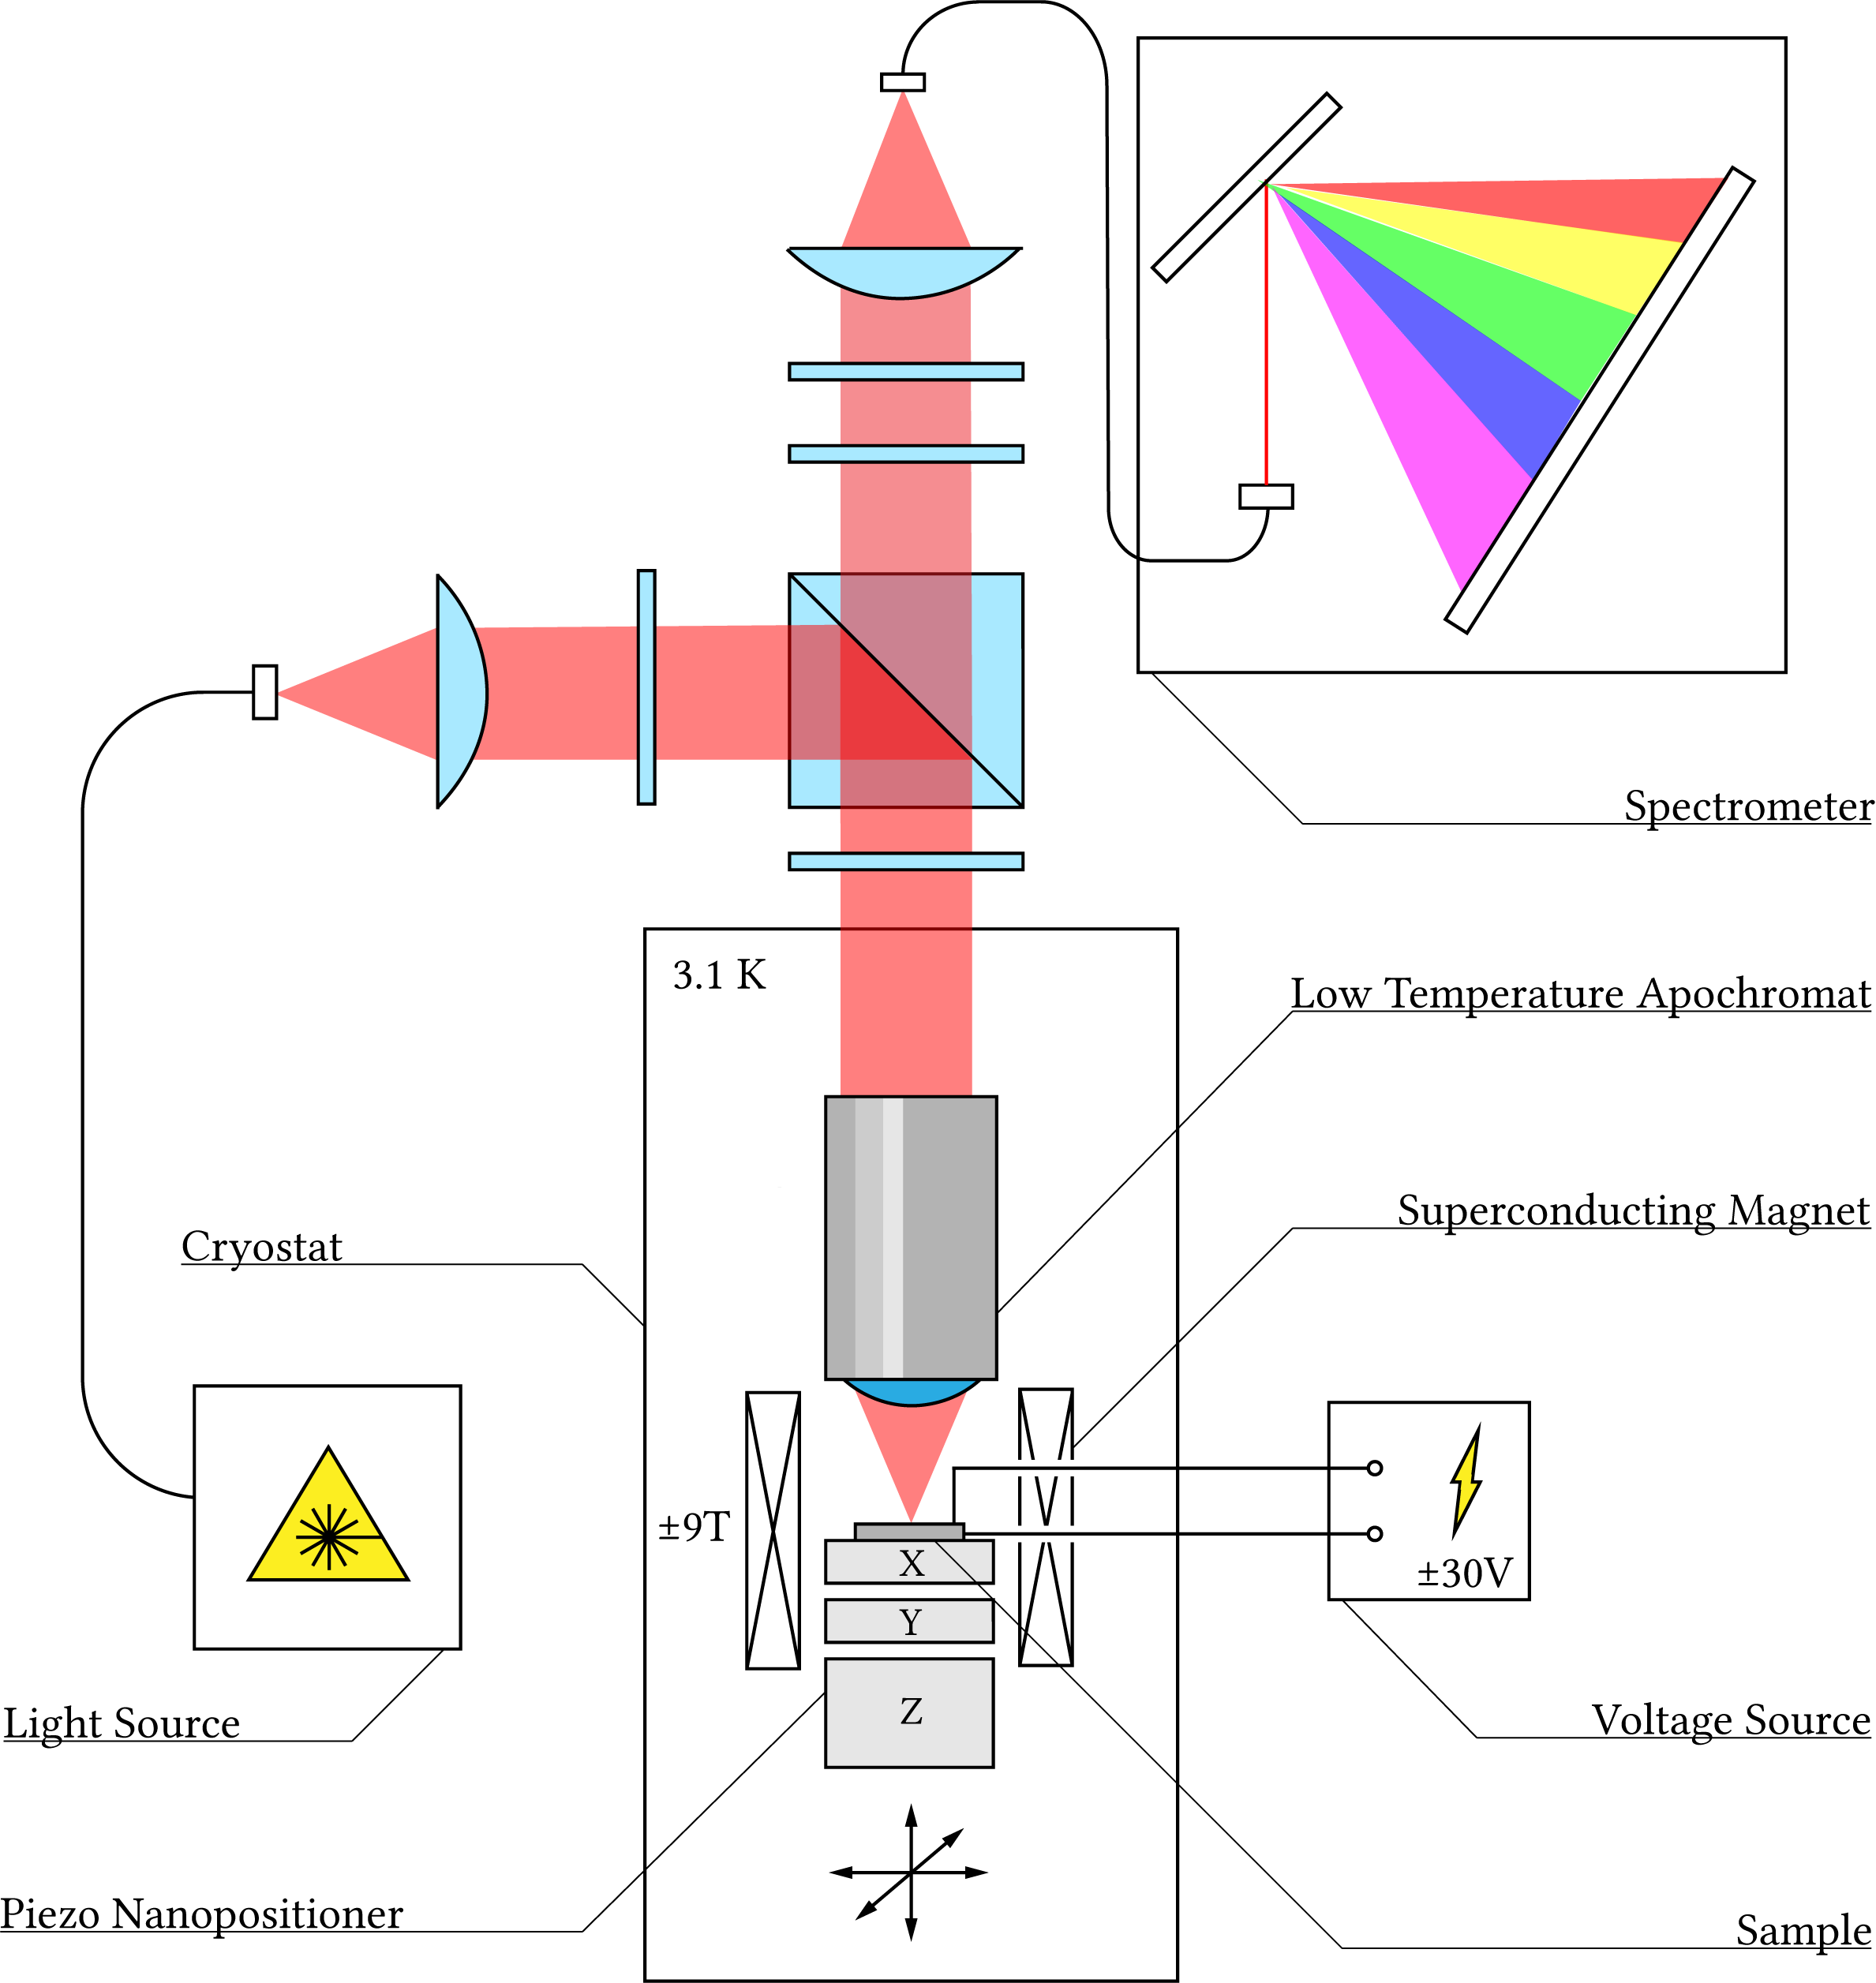
\includegraphics[width=.8\textwidth]{OptischerAufbau.png}
	\caption{Optical setup for confocal spectroscopy: Light from a \textbf{laser}-source is guided to the setup in a single mode opical fibre and collimated. To cut off raman-modes, that are created in the fibre a \textbf{shortpass} filter is installed behind the collimator. A \textbf{linear polarizer} defines a polarization axis. A \textbf{beam-sampler} is reflecting the excitation beam into a \textbf{low temperature apochromat}, whose focus lies on the sample, with a spotsize of \textasciitilde\- 0.5\mu m. The sample is mounted on a \textbf{piezo nanopositioner}, that is placed inside a \textbf{cryostat} at a temperature of up to 3.1 K or in a container of liquid helium at 4.2 K. The cryostat is equipped with a \textbf{superconducting magnet} that can supply a homogenious magnetic field up to 9T. The sample electrodes are connected to a \textbf{voltage source} (Yokogawa) that supplies {\small$\pm$}32V. The detection spot is identical with the excitation. The reflection or photoluminescence is collimated again in the objective and passes through a \sigma$^+$/\sigma$^-$-analyzer consisting of a \textbf{quarter waveplate} and a \textbf{linear polarizer}, before being focussed in the detection fibre that connects to a \textbf{spectrometer}. A \textbf{camera} can be used to monitor the spot and image the sample, if it is brought out of focus.}
	\label{opticalsetup}
\end{figure}

The optical setup is a confocal microscope. In contrast to a ``conventional'' microscope, the sample is placed in the focal plane of a low temperature objective. The focal point is the same for excitation of the sample and the detection of the reflection or photoluminescence signal, hence the name. A scheme of the complete setup can be seen in Figure \ref{opticalsetup}. The excitation beam from a laser is guided to the so called excitation arm with a single mode optical fibre. It passes though a linear plolarizer to define a polarization axis and is reflected to the objective by a beam-sampler. To analyze the mostly circularly polarized light of the detection beam, it passes through a quarter waveplate and another linear polarizer and is focussed into another optical fibre, that is connected to a spectrometer. The sample is mounted on a piezo nanopositioner inside a cryostat or can of liquid helium and connected to a voltage source, to tune the charge density in the \tmdg flake. A strong, homogenious magnetic field can be supplied by a superconducting magnet.

For photoluminescence spectroscopy, the sample is excited with a laserbeam with a narrow frequency profile and a higher intensity. Because this beam has a much higher intensity, than the collected \textsc{pl} it is tuned to a higher frequency than the main exiton resonance. A shortpass filter in the excitation arm makes sure, no raman modes from the optical fibre pollute the spectrum. A longpass filter, right before the optical fibre of the detection arm blocks the laser, so that only \textsc{pl} reaches the spectrometer. To optain a reflection spectrum, these filters are omitted. Instead, the sample is illuminated with a broad band light source at a low power. To find the signal, a background spectrum, recorded in absence of the \tmdg flake is substracted from the main spectrum.

\[ 
	S_R = \frac{\Delta R}{R} = \frac{R_{\mathrm{flake}} - R_{\mathrm{background}}}{R_{\mathrm{background}}}
\]

The signal $S_R$ is the difference of the Reflection signals of \tmdg flake and background. The devision by the background reflection is made to normalize the signal. The resulting reflection spectrum should show only features, of the flake. In practice, the obtained data has to be evaluated with some precautions in mind, to avoid misidentifiying for example interference effects due to differences in \hbng thickness as features of the absorption behaviour of the sample.

\section{Sample characterization}

There are two dimensions to characterize the quality of a sample. Its optical properties must include narrow linewidths, to identify different features of the spectrum and it has to be gate-tunable, which means the contact of \tmdg flake to the electrode as well as the backgate have to function and the \sio layer has to sustain enough voltage to tune in and out of neutral and charged regimes.

\section{Electrical characterization}

To function of a gate-tunable \tmd-device is threefold. The top-gate electrode has to be in contact with the flake of interest, the contacts to the backgate have to function, especially at low temperature and the dielectric has to hold enough voltage to see effects in the optical spectrum. Because the flake has only one contact, no transport measurement is possible. Hence the quality of the top-gate contact can only be assessed by seing its effects in the optical spectrum. The other two criteria can be checked and quantified without any optical means. As mentioned in (Section vong 1 fabrikation) the p-doped silicon bulk material, that is used as the back-gate electrode is prepared with two contacts. Both of these contacts can be connected to a simple multimeter, to measure the resistance between them. For this particular material a resistance of 5-6 \Omega\ means, the contacts function as planned. If there is no contact or a high resistance, one of the contacts might still be functional. This can be assessed by observing the spectrum for different voltages, just like the top-gate. Nevertheless, having an additional check by using two back-gate contacts, helps troubleshooting in case of issues with the device.

The quality of the dielectric is quantified by measuring the capacity of the device for different voltages and monitoring the leak current (see Figure CV). A constant voltage across the desired range of operation ({\small$\pm $}30V) is added to a small alternating current of small amplitude ($U_0 = $ 10 mV$_{pp}$, $f = $ 77.1 Hz). The real part of the resulting current is the resistive current, or leakage and the imaginary part is proportional to the capacity. Both parts can be measured in a lock-in amplifier. For our devices, the leakage current at low voltages should not exceed the pico-ampere range. For characterizing the dielectric the constant voltage can be raised until the resistive current starts rising exponentially. The corresponding voltage is the maximum, that should be applied in the particular sample, because a higher voltage can result in charges breaking through the dielectric and forming conducting chanels, thus disabling the gate-tunability permanently. This sensitivity is the reason to use this more complicated characterization method instead of simply monitoring the current while applying voltages directly. Because very low currents can be measured with the lock-in amplifier, the boundary of safe operation can be approached very carefully.

%Here is a figure of CV-measurement

\section{Spectral resolution}
\subsection{Spectral features at different doping levels}

\begin{figure}
	\begin{subfigure}{0.49\textwidth}
		\caption{}
		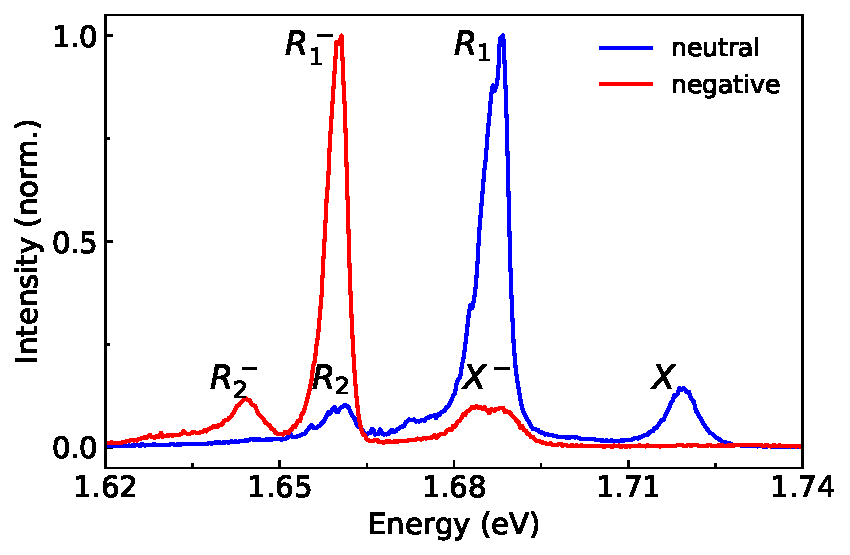
\includegraphics[height=0.65\textwidth]{spectrum_neutral_negative}
	\end{subfigure}
	\begin{subfigure}{0.49\textwidth}
		\caption{}
		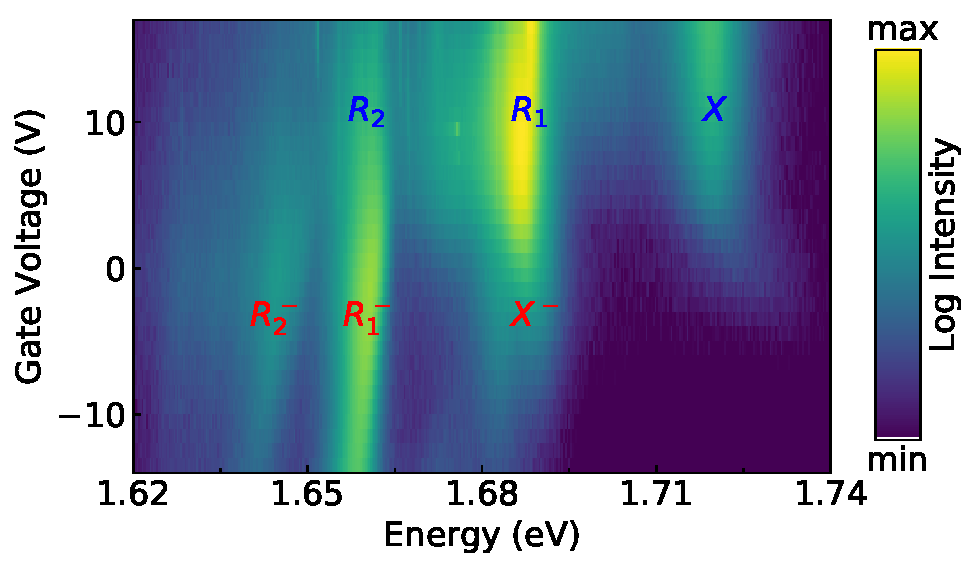
\includegraphics[height=0.65\textwidth]{Voltsweep}
	\end{subfigure}
\end{figure}

%\subsection{Measuring the valley zeeman effect}

%\begin{appendices}
%\end{appendices}
\printbibliography
\end{document}